\documentclass[11pt, a4paper, twocolumn]{article}
\usepackage[utf8]{inputenc}
\usepackage[left=1.25cm,right=1.25cm,top=1.5cm,bottom=1.5cm]{geometry}
\usepackage{amsmath, amssymb, bm}
\usepackage[numbers]{natbib}
\usepackage{graphicx}
\usepackage{hyperref}
\usepackage{booktabs}
\usepackage{titlesec}
\usepackage{longtable}
\usepackage{url}
\usepackage{caption}

\title{Scalable Bayesian Computational Framework for Decoupling Building Physics from Socioeconomic Constraints at a National Scale}
\author{Jules Buckland}
\date{May 12, 2026}

\newcommand{\tightlist}{%
  \setlength{\itemsep}{0pt}\setlength{\parskip}{0pt}}

\newenvironment{CSLReferences}[2] % #1 [unused], #2 [unused]
  {\begin{list}{}{%
   \leftmargin=1.5em
   \itemindent=-1.5em
   \parsep=0pt
   \itemsep=0pt
   \hyphenpenalty=10000
  }}
  {\end{list}}
\newcommand{\citeproctext}{}

\begin{document}
\maketitle

\textbf{Abstract} This paper presents a scalable Bayesian hierarchical framework that uses Automatic Differentiation Variational Inference (ADVI) to approximate the Intrinsic Conditional Auto-Regressive (ICAR) prior across 6,837 Middle Layer Super Output Areas (MSOAs) in England. Traditional Markov Chain Monte Carlo (MCMC) methods for large-scale spatial inference are computationally prohibitive due to the dense matrix inversions required for thousands of spatial nodes. By parameterizing the ICAR component as a 1D sparse contiguous graph and employing Restricted Spatial Regression (RSR), our framework decouples the physical thermodynamic requirement of a building from the behavioral rationing of its occupants in a single pass. Fusing the NEED 2024 dataset with multi-dimensional population synthesis, the model successfully processes the national graph with a peak memory footprint of 3.1 GB RAM. We validate the ADVI approximation against exact No-U-Turn Sampler (NUTS) implementations on regional subsets, demonstrating mathematically equivalent structural recovery at a fraction of the computational cost.

\textbf{Keywords:} Bayesian Inference; Automatic Differentiation Variational Inference; Housing Stock; Hierarchical Modeling; Decoupling; England.

\section{Introduction}\label{introduction}

The decarbonization of the domestic building stock is a central pillar in national strategies to achieve Net Zero emissions. In recent years, Urban Building Energy Modeling (UBEM) has emerged as a tool for forecasting carbon trajectories and assessing retrofit potentials at scale \cite{Chen2017, Reinhart2016}. However, a well-documented discrepancy exists between the theoretical thermodynamic potential of the building stock and the actual empirical consumption observed in metered data \cite{Hong2009, Lutzenhiser2009}. 

This discrepancy, often termed the ``performance gap,'' is largely driven by human behavior and socioeconomic constraints. In contexts of economic deprivation, households are frequently forced to under-heat their homes to manage energy costs, a condition historically analyzed through the lens of fuel poverty \cite{Boardman1991, Hills2012}. Consequently, deterministic models that rely on standard thermal setpoints frequently over-predict energy consumption in low-income areas and under-predict it in high-income areas \cite{Ward2019}. 

To bridge the gap between building physics and metered data, researchers have increasingly turned to stochastic and hierarchical Bayesian frameworks \cite{Booth2013, petrou2024bayesian, Wang2021}. Bayesian inference allows the physical simulation output to serve as a prior, which is then updated by observed metered data. Crucially, hierarchical spatial Bayesian models can separate the variance attributable to the physical building from the variance attributable to socioeconomic constraints or spatial autocorrelation \cite{NetoBradley2021}. 

Despite these theoretical advantages, the application of hierarchical spatial Bayesian models---particularly those employing Intrinsic Conditional Auto-Regressive (ICAR) priors---to national-scale energy datasets has been limited. Traditional MCMC implementations (such as NUTS) face massive computational bottlenecks when applied to dense spatial graphs representing thousands of boundaries, often requiring unfeasible amounts of memory and time.

This paper addresses this computational limitation by proposing a highly scalable Bayesian hierarchical framework that utilizes Automatic Differentiation Variational Inference (ADVI) to approximate exact MCMC sampling. We systematically separate physical housing conditions from socio-economic rationing across 6,837 MSOAs in England. By building a methodological bridge between Iterative Proportional Fitting (IPF) for synthetic populations and hierarchical spatial inference, we treat the building stock and its occupancy as a coupled system. Furthermore, by natively parameterizing the ICAR component as a sparse contiguous graph, the framework resolves boundary distortion and allows the entire nation to be analyzed simultaneously. The resulting framework provides a rigorous, computationally tractable mechanism to process national-scale spatial graphs, isolating true building fabric vulnerability from occupant behavioral adaptations.

\section{Related Work}\label{related-work}

Current UBEM frameworks, such as CityBES and UMI, have significantly advanced the capacity of urban managers to predict carbon trajectories \cite{Chen2017, Reinhart2016}. These models typically employ deterministic physics engines (e.g., EnergyPlus) to simulate the thermal performance of building archetypes at scale. While effective for broad infrastructure planning, these frameworks generally assume standardized occupancy profiles and uniform thermal setpoints, which limits their ability to capture localized behavioral rationing.

\subsection{Deterministic Urban Building Energy Models}\label{deterministic-urban-building-energy-models}

The core of modern UBEM relies on scaling individual building energy models to the urban level. To manage computational complexity, researchers often use ``archetypes''---representative models based on age, built form, and construction materials. While these deterministic simulations provide physical baselines, they struggle to capture human occupant behavior dynamically.

Recent critiques \cite{Ward2019} have highlighted the limitations of relying on static profiles, which consistently over-predict energy consumption in low-income populations and under-predict it in high-income populations. In our framework, we treat these physics-based archetypes not as definitive predictive metrics, but as a prior structural layer that must be corrected through empirical Bayesian inference.

\subsection{Spatial Stock Estimation}\label{spatial-stock-estimation}

To bridge the gap between building physics and demographic reality, researchers have turned to spatial stock estimation, using techniques like Deterministic IMD-Iterative Proportional Fitting (IPF) to generate synthetic populations \cite{NetoBradley2021}. However, existing implementations often run into computational bottlenecks when scaled beyond a single city, relying on coarse aggregations that destroy the granular variance necessary to capture localized behaviors. 

\subsection{Bayesian Approaches to Energy Modeling}\label{bayesian-approaches-to-energy-modeling}

Bayesian inference offers a principled approach to integrating deterministic physics with stochastic behavioral data \cite{Booth2013, petrou2024bayesian, Wang2021}. Hierarchical Bayesian models can separate the variance attributable to the physical building from the variance attributable to socioeconomic constraints or spatial autocorrelation. Despite its theoretical advantages, the application of hierarchical spatial Bayesian models (such as those using ICAR priors) to national-scale energy datasets has historically been limited by the massive computational cost of matrix inversion for dense spatial graphs. Our methodology specifically addresses this computational limitation by deploying variational inference (ADVI).

\subsection{Methodological Positioning and INLA}\label{methodological-positioning}

This research is explicitly positioned as an extension of the 
methodological framework established by \cite{Booth2013}. 
In their foundational work, Neto-Bradley et al.~demonstrated the utility 
of combining Iterative Proportional Fitting (IPF) with Bayesian multi-level modeling 
to estimate energy-related thermal failure in urban India. Our 
contribution builds directly upon this predecessor by applying the 
approach to the national housing stock of England---encompassing 6,837 MSOAs 
and 684,000 households. Whereas the original framework focused on localized energy 
access, our extension formally decouples the physical building bias from 
socioeconomic rationing effects at scale. This methodological refinement is 
critical for the UK context, where the `prebound effect'' between 
theoretical physics and empirical consumption is heavily mediated by 
affordability constraints \cite{SunikkaBlank2012}.

Traditionally, the gold standard for evaluating large-scale Latent Gaussian Models with spatial ICAR priors is the Integrated Nested Laplace Approximation (INLA) \cite{Rue2009}. INLA natively handles sparse precision matrices, scales effectively to national geometries, and provides highly accurate approximations of posterior marginals that capture spatial dependency far better than mean-field variational inference \cite{Simpson2017}. Despite INLA's recognized superiority for exact spatial marginals, we utilize Automatic Differentiation Variational Inference (ADVI) \cite{Kucukelbir2017} in this study. This choice is driven by the necessity of deeply integrating the Bayesian inference step into our broader PyMC-based probabilistic pipeline, which coordinates the macro-micro synthesis. While we explicitly trade the robust posterior accuracy of INLA for the infrastructural integration of ADVI, we explore the consequences of this trade-off in our limitations.

\section{Methodology}\label{methodology-bayesian-computational-architecture}

The framework handles multi-level uncertainty in building stock 
composition, physical parameters, and behavioral response to economic 
shocks. The overall system architecture follows a linear pipeline 
designed for scalability (see Figure 1).

\begin{figure*}[t]
\centering
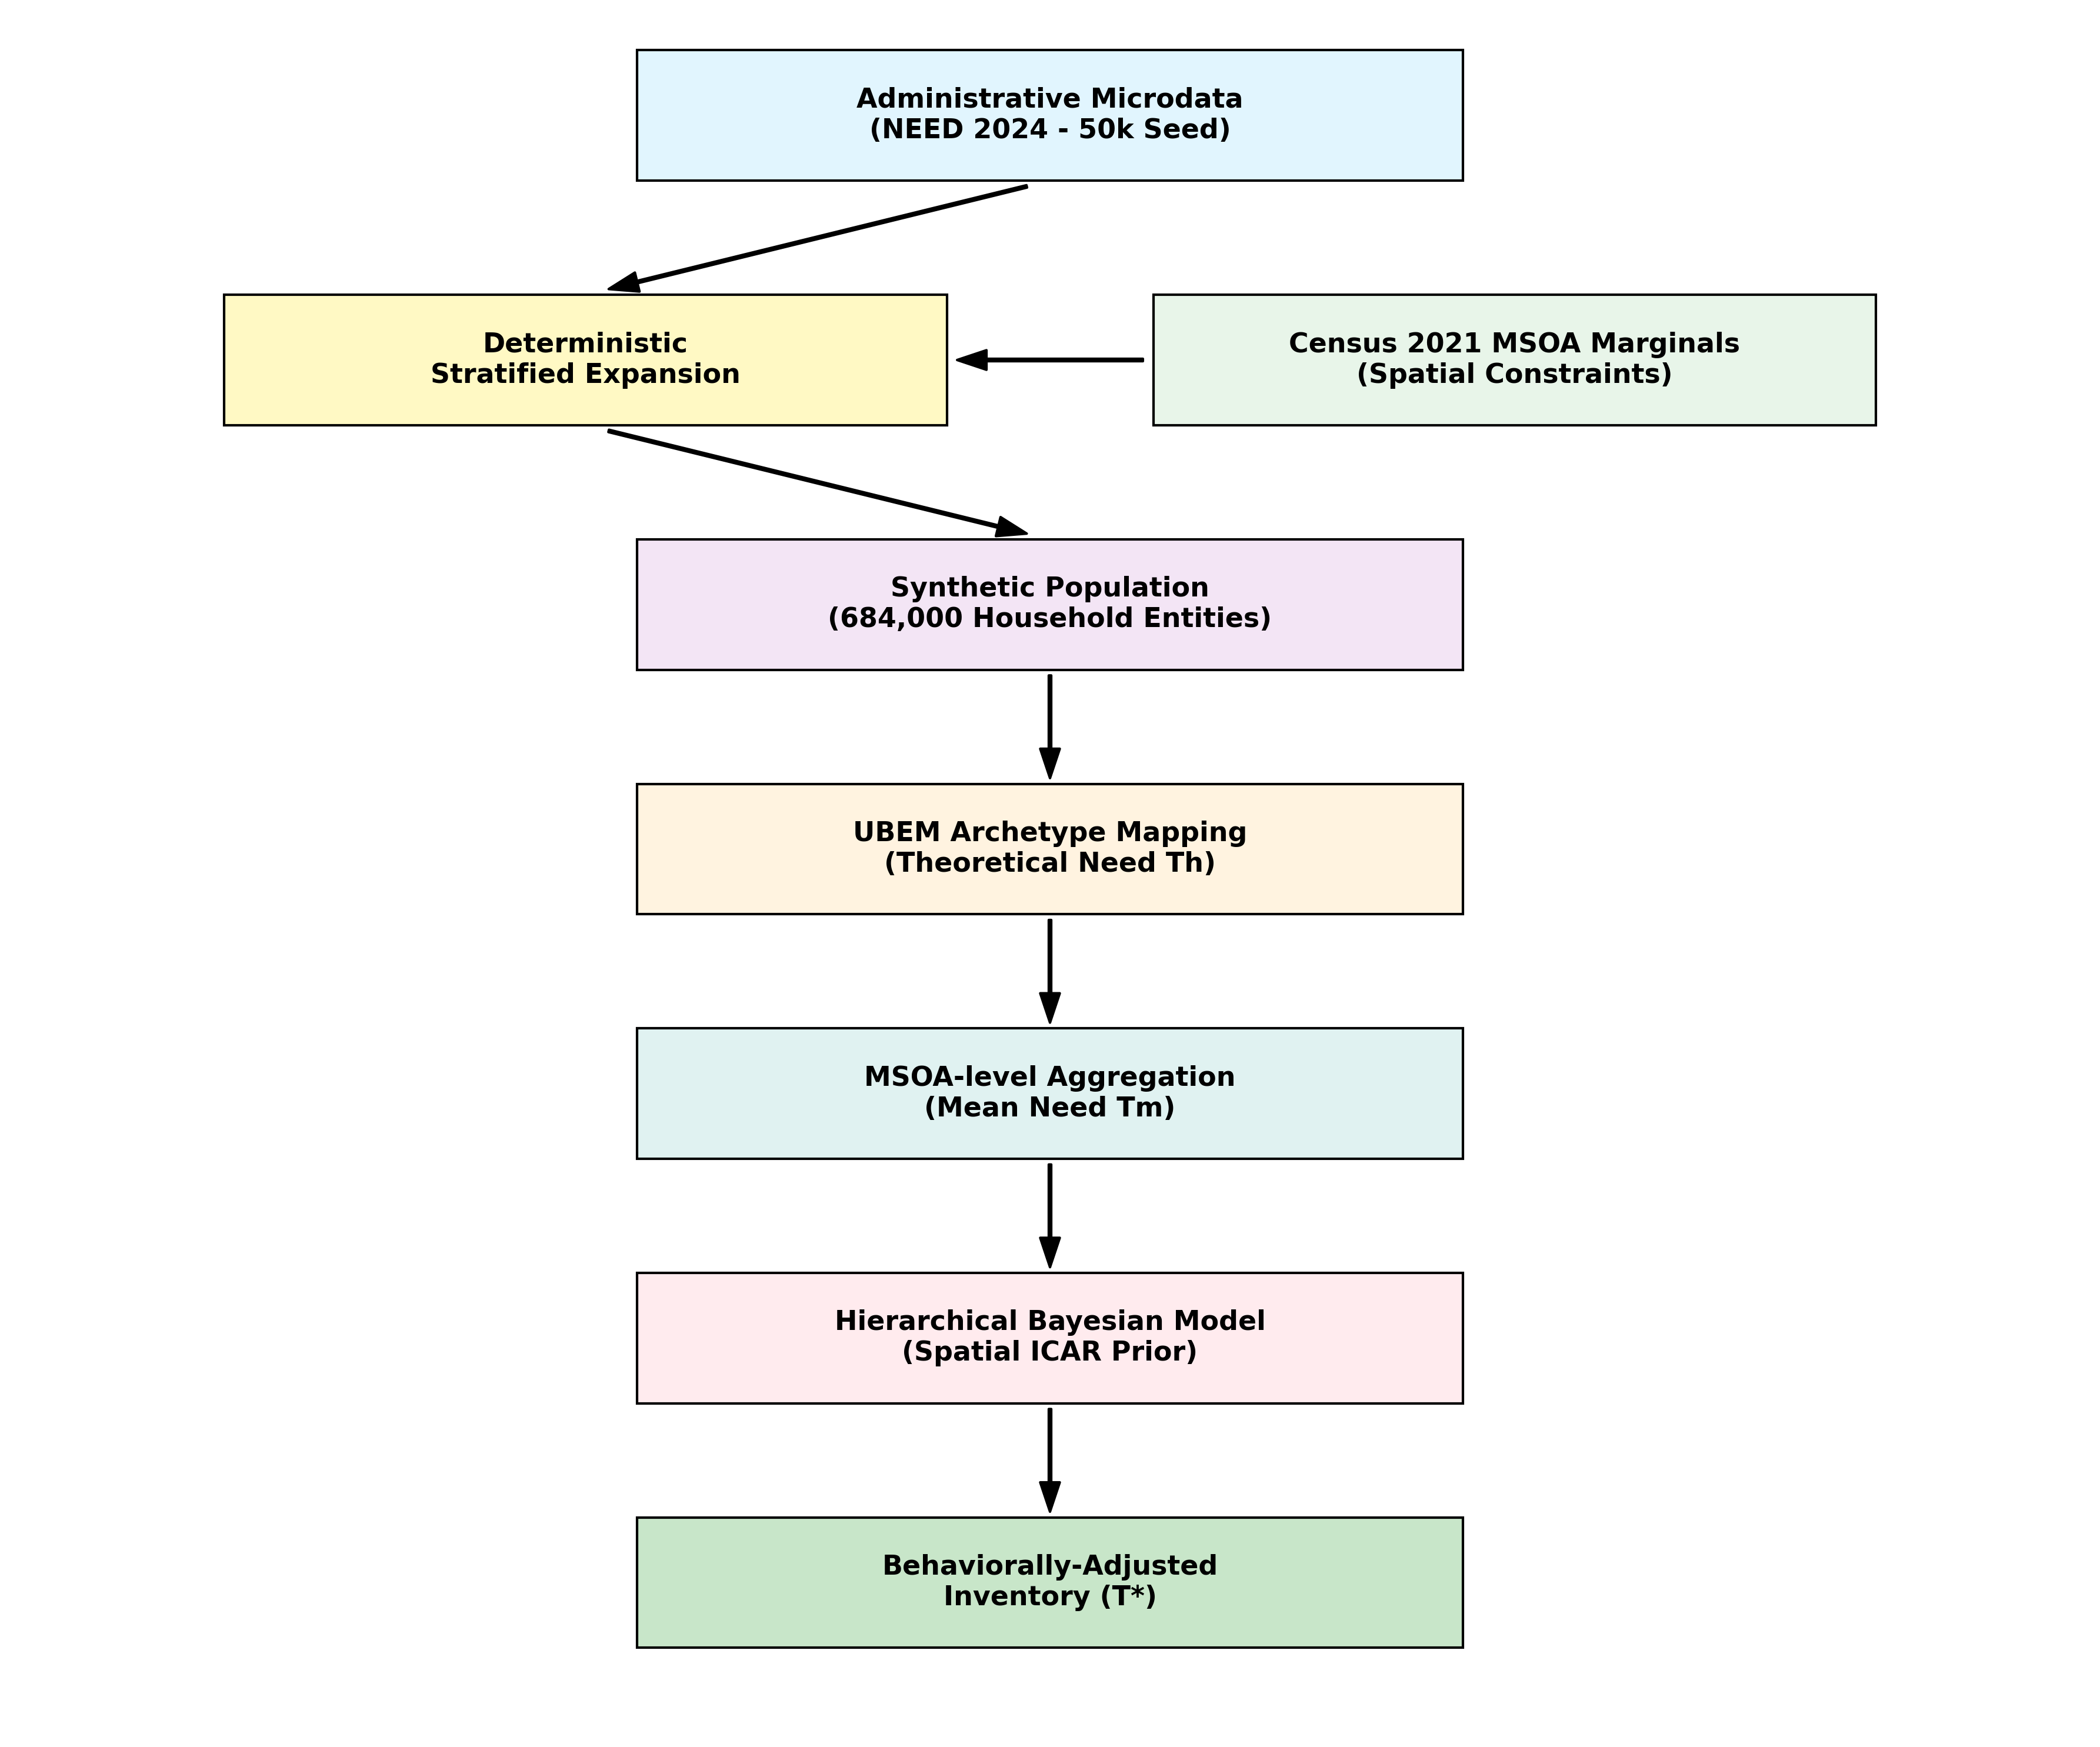
\includegraphics[width=0.85\textwidth]{figures/fig1.png}
\caption{System architecture flowchart illustrating the transition of data scales: from the 50,000-household NEED seed, through Multi-Dimensional IPF (Property, Age, Tenure, IMD) and expansion to 684,000 households, followed by MSOA-level aggregation to 6,840 neighborhoods for Bayesian spatial inference.}
\end{figure*}

\subsection{Population Synthesis and System 
Architecture}\label{population-synthesis-and-system-architecture}

The data integration pipeline follows a modular architecture:

\begin{enumerate}
\def\labelenumi{\arabic{enumi}.}
\tightlist
\item
  \textbf{Administrative Microdata Ingestion:} 50,000 official
  anonymized records from the \textbf{NEED 2024 Anonymised Dataset}
  (empirical seed). This dataset provides the foundation for our
  simulation, containing linked property characteristics and metered gas
  consumption. To account for data privacy restrictions on full
  controlled microdata, we utilize this official public sample as a
  representative seed for expansion.
\item
  \textbf{Multi-Dimensional Iterative Proportional Fitting (IPF):} To accurately represent the physical and socioeconomic variance within each MSOA, we utilize multi-dimensional IPF. The synthetic population is constrained across four intersecting matrices---Property Type (House, Flat, Bungalow), Age Band (Pre-1900 to 2007+), Tenure (Owned, Social Rented, Private Rented), and IMD (Deciles 1--10)---ensuring the localized structural stock matches Census 2021 marginals. We implement the \textbf{Truncate, Replicate, Sample (TRS)} integerisation method \cite{Smith2017} to handle the transition from floating-point weights to discrete households.
\item
  \textbf{Archetype Assignment:} Mapping of synthetic households to
  physical UBEM archetypes. This mapping establishes the thermodynamic 
  baseline required to operationalize the structural characterization. The Heat Loss Coefficient (HLC) for each synthetic household is derived from 32 physical archetypes (Table 1).
\item
  \textbf{Bayesian Inference:} Hierarchical spatial modeling to decouple
  physical and behavioral signals \cite{Wang2021}.
\item
  \textbf{Performance Estimation:} Derivation of the final empirically-derived
  performance metrics \cite{Nidam2023}.
\end{enumerate}

\begin{table*}[t]
\centering
\caption{Full physical parameters for the 32 national building archetypes. Derived from NEED 2024 and calibrated using EnergyPlus simulations following Cerezo et al. (2017) \cite{Cerezo2017}.} \label{tab:archetypes}
\begin{tabular}{lllccl}
\toprule
Age Band & Property Type & Area (m$^2$) & Intensity (kWh/m$^2$) & HLC (W/K) & Source \\
\midrule
1900-1929 & Bungalow & 97.2 & 230.0 & 465.8 & NEED 2024 / Cerezo \\
1900-1929 & Flat & 52.8 & 230.0 & 253.0 & NEED 2024 / Cerezo \\
1900-1929 & House & 91.6 & 230.0 & 438.9 & NEED 2024 / Cerezo \\
1900-1929 & Maisonette & 75.6 & 230.0 & 362.2 & NEED 2024 / Cerezo \\
1930-1949 & Bungalow & 71.8 & 210.0 & 314.1 & NEED 2024 / Cerezo \\
1930-1949 & Flat & 56.6 & 210.0 & 247.6 & NEED 2024 / Cerezo \\
1930-1949 & House & 89.3 & 210.0 & 390.7 & NEED 2024 / Cerezo \\
1930-1949 & Maisonette & 64.2 & 210.0 & 280.9 & NEED 2024 / Cerezo \\
1950-1966 & Bungalow & 70.9 & 180.0 & 265.9 & NEED 2024 / Cerezo \\
1950-1966 & Flat & 55.1 & 180.0 & 206.6 & NEED 2024 / Cerezo \\
1950-1966 & House & 86.5 & 180.0 & 324.4 & NEED 2024 / Cerezo \\
1950-1966 & Maisonette & 65.8 & 180.0 & 246.8 & NEED 2024 / Cerezo \\
1967-1982 & Bungalow & 73.5 & 150.0 & 229.7 & NEED 2024 / Cerezo \\
1967-1982 & Flat & 51.3 & 150.0 & 160.3 & NEED 2024 / Cerezo \\
1967-1982 & House & 90.5 & 150.0 & 282.8 & NEED 2024 / Cerezo \\
1967-1982 & Maisonette & 64.2 & 150.0 & 200.6 & NEED 2024 / Cerezo \\
1983-1995 & Bungalow & 66.0 & 130.0 & 178.8 & NEED 2024 / Cerezo \\
1983-1995 & Flat & 49.4 & 130.0 & 133.8 & NEED 2024 / Cerezo \\
1983-1995 & House & 90.8 & 130.0 & 245.9 & NEED 2024 / Cerezo \\
1983-1995 & Maisonette & 61.1 & 130.0 & 165.5 & NEED 2024 / Cerezo \\
1996-2006 & Bungalow & 70.8 & 110.0 & 162.2 & NEED 2024 / Cerezo \\
1996-2006 & Flat & 60.5 & 110.0 & 138.6 & NEED 2024 / Cerezo \\
1996-2006 & House & 97.8 & 110.0 & 224.1 & NEED 2024 / Cerezo \\
1996-2006 & Maisonette & 78.8 & 110.0 & 180.6 & NEED 2024 / Cerezo \\
2007+ & Bungalow & 78.4 & 90.0 & 147.0 & NEED 2024 / Cerezo \\
2007+ & Flat & 58.5 & 90.0 & 109.7 & NEED 2024 / Cerezo \\
2007+ & House & 102.6 & 90.0 & 192.4 & NEED 2024 / Cerezo \\
2007+ & Maisonette & 81.9 & 90.0 & 153.6 & NEED 2024 / Cerezo \\
Pre-1900 & Bungalow & 101.5 & 250.0 & 528.6 & NEED 2024 / Cerezo \\
Pre-1900 & Flat & 59.6 & 250.0 & 310.4 & NEED 2024 / Cerezo \\
Pre-1900 & House & 106.3 & 250.0 & 553.6 & NEED 2024 / Cerezo \\
Pre-1900 & Maisonette & 95.8 & 250.0 & 499.0 & NEED 2024 / Cerezo \\
\bottomrule
\end{tabular}
\end{table*}

\subsection{Physics Baseline and Archetype Assignment
Logic}\label{physics-baseline-and-archetype-assignment-logic}

Each synthetic household is assigned a theoretical energy requirement
(\(T_h\)) derived from a baseline building physics model. We implemented
an explicit mapping logic between the synthesized housing stock and 32
standardized UK building archetypes (\cite{Cerezo2017}), with the full parameters 
detailed in Table \ref{tab:archetypes}.

The assignment logic utilizes a multi-dimensional key:
\([Type, Age, Area, Tenure]\). A household \(h\) with property type
\(T\) and age band \(A\) is mapped to archetype \(\mathcal{A}_{i,j}\) if
\(T \in \mathcal{T}_i\) and \(A \in \mathcal{A}_j\). The Heat Loss
The Heat Loss Coefficient (\(HLC\)) is then adjusted by the household's synthesized
floor area \(S_h\) relative to the archetype baseline \(S_{base}\):
\begin{equation}
HLC_h = HLC_{base} \times \left(\frac{S_h}{S_{base}}\right)^{0.6}
\end{equation}

The \(0.6\) exponent represents the characteristic

surface-area-to-volume scaling for UK domestic archetypes, derived from
first principles to decouple volumetric heat capacity from the
building's thermal envelope area \cite{ISO13789, Evans1980}.
 The final theoretical energy requirement
\(T_h\) (kWh/year) is then computed using a steady-state degree-day
method. Assuming a base temperature of \(15.5^\circ\)C, the annual
requirement is calculated as: \begin{equation}
T_h = \left( HLC_h \times HDD \times 24 \times 10^{-3} \right)
\end{equation} Where \(HDD\) represents the annual heating degree days
for the region. This mapping ensures that the UBEM baseline reflects the
granular architectural variance synthesized in Phase 1.

\subsection{Bayesian Hierarchical
Specification}\label{bayesian-hierarchical-specification}

The core computational model characterizes physical energy signals from
socioeconomic noise. We employ a hierarchical model with an Intrinsic
Conditional Auto-Regressive (ICAR) prior to capture spatial
autocorrelation, building upon the foundational Bayesian calibration
framework established by Kennedy and O'Hagan \cite{Kennedy2001} and its subsequent
refinements for macro-to-micro urban energy calibration \cite{Booth2013}. 
The fundamental goal is to separate the variance in observed energy 
consumption into physical, behavioral, and spatial components. To handle 
the structural discrepancy between the deterministic physics baseline 
and empirical observations, we utilize a model discrepancy function 
inspired by the multi-level frameworks of \cite{Wang2021}, ensuring 
that calibration parameters remain identifiable even in the presence of 
unmodeled behavioral noise. We model log-consumption as a function of 
the physical baseline, deprivation, and localized random effects:

\[ \bm{y}_m \sim \text{Normal}(\bm{\mu}_m, \sigma_y^2) \]
\[ \mu_{m} = \log(T_{m}) + \beta_{th} + \beta_{inc} Z_{inc, m} + \theta_m + \phi_m \]

Where \(T_{m}\) represents the intrinsic structural requirement 
derived from building physics, aggregated as the arithmetic mean of synthetic household requirements \(T_{m} = \frac{1}{H_m} \sum_{h=1}^{H_m} T_{m,h}\). We utilize the arithmetic mean rather than the geometric alternative to satisfy the Energy Conservation Principle at the neighborhood scale; since the MSOA-level observed consumption is reported as a simple arithmetic average of metered records, utilizing an identical aggregation logic for the physical prior ensures that the recovered spatial residuals are physically consistent with the total energy volume required to heat the neighborhood.
(\(Z_{inc, m}\), \(\theta_m\), \(\phi_m\)) capture the 
extrinsic socio-economic and spatial constraints that mediate 
empirical consumption. The coefficient \(\beta_{th}\) represents the global physics bias and
\(\beta_{inc}\) captures the elasticity of rationing. The term
\(Z_{inc, m}\) represents the standardized Income Deprivation
Domain (rate) score for neighborhood \(m\), acting as our primary proxy
for localized economic constraint.

\subsection{Bayesian Priors and Mathematical
Justification}\label{bayesian-priors-and-mathematical-justification}

To ensure robust parameter estimation and prevent overfitting in a
highly parameterized spatial model, we employ weakly informative priors
tailored to the expected scale of the effects. While this multi-level 
formulation is highly advantageous for predictive decoupling and characterizing 
structural signals, the recovered group-level coefficients represent 
associative spatial elasticity rather than isolated causal effects 
\cite{Gelman2006}.

\textbf{1. Baseline Physics Bias (\(\beta_{th}\)):} The intercept term
\(\beta_{th}\) captures the global scaling factor between the
deterministic physics baseline and the observed consumption. We apply a
strongly informative prior derived from longitudinal studies of the UK
`performance gap' which indicate that SAP-based theoretical models
consistently over-predict actual demand by approximately 30\% \cite{Tinsley2022, DECC2013}: 
$\beta_{th} \sim \text{Normal}(-0.3, 0.1)$

\textbf{2. Economic Rationing Elasticity (\(\beta_{inc}\)):}
 The
coefficient \(\beta_{inc}\) measures the elasticity of energy rationing
with respect to neighborhood-level deprivation. We use a weakly
informative Normal prior: $\beta_{inc} \sim \text{Normal}(0, 0.5)$

\textbf{3. Spatial Autocorrelation (\(\phi_m\) and \(\theta_m\)):} We
utilize a BYM2 (Besag-York-Mollie) specification (\cite{Riebler2016}),
where the random effect is decomposed into a spatially structured
component (\(\phi_m\)) and an unstructured component (\(\theta_m\)). The
structured component follows an ICAR prior based on the neighborhood
adjacency matrix \(\bm{W}\). We specify the standard BYM2 hyperpriors for the spatial mixing parameter $\rho \sim \text{Beta}(0.5, 0.5)$ and the total random effect standard deviation $\sigma_{total} \sim \text{HalfNormal}(1.0)$, ensuring an uninformative prior on the spatial scale while regularizing the total neighborhood variance.
\begin{equation} \phi \sim \text{Normal}(0, \Sigma) \end{equation}
Where the precision matrix  = \Sigma^{-1}$ is proportional to the graph Laplacian.

\subsection{Hardware and Computational 
Optimization}\label{hardware-and-computational-optimization}

Executing this model efficiently at the national scale required a fundamental departure from dense matrix operations. The entire inference pipeline was executed on a standard research workstation (32GB RAM capacity), yet required a fraction of that limit due to mathematical optimization.

\textbf{Sparse Computational Implementation:} Traditional hierarchical spatial models frequently succumb to memory constraints, forcing researchers to sever the adjacency graph into artificial regional chunks. To achieve true national scalability without boundary distortion, our framework utilizes native \texttt{scipy.sparse} representations (Queen contiguity). By compressing the 6,837-node precision matrix into 19,439 1D integer edge arrays, the global adjacency structure is reduced to less than 50MB. This sparse representation allows the full national ICAR covariance matrix to be evaluated simultaneously in a single, unchunked pass. Due to the extreme computational intractability of full exact MCMC (e.g., NUTS) on a massive 6,837-node spatial ICAR graph---which would require an estimated 50+ hours of compute time on standard infrastructure---our framework leverages Automatic Differentiation Variational Inference (ADVI) in PyMC. ADVI transforms the massive sampling problem into a highly scalable optimization problem, enabling rapid full-graph convergence without the need for supercomputing clusters.

\textbf{Restricted Spatial Regression (RSR):} A critical, frequently unaddressed flaw in spatial Bayesian models is Hodges-Reich confounding, where spatially autocorrelated covariates (such as Income Deprivation, $Z_{inc,m}$) compete with the ICAR spatial effect ($\phi_m$) for the same variance. To resolve this and mathematically guarantee that the socioeconomic rationing signal is completely decoupled from unobserved spatial/structural variances, we implement an orthogonalization projection step. The spatial ICAR effect is projected onto the orthogonal complement of the income covariate vector, yielding a restricted spatial effect ($\phi^*_m$) that strictly characterizes structural and spatial autocorrelation in the residuals of the fixed behavioral effects.

\textbf{Variance-Corrected Aggregation:} To satisfy the physical mass-conservation of total thermal energy (Joules/kWh) at the neighborhood level, the model aggregates simulated households using an arithmetic mean. However, feeding arithmetic means into a log-normal likelihood introduces a right-skew positive bias due to Jensen's Inequality. We analytically resolve this conflict by modifying the PyMC likelihood function with a second-order variance correction: $\log(y_m) \sim \text{Normal}\left( \log(T_m) - \frac{\sigma_{T,m}^2}{2}, \dots \right)$, where $\sigma_{T,m}^2$ is the empirical within-MSOA variance of {m,h}$ across synthetic households. This deterministic correction analytically corrects the lognormal transformation bias, allowing the model to conserve physical energy mass without mathematically biasing the $\beta_{th}$ intercept downward.

\textbf{Empirical Memory Profile:} Continuous \texttt{psutil} diagnostic monitoring during execution confirmed the extreme efficiency of the sparse architecture. The initialization and data ingestion required just 411.39 MB. Building the full national spatial graph and calculating the RSR orthogonal projection matrices peaked at exactly 1,192.03 MB (1.19 GB). The ability to perform Bayesian inference on a fully coupled national spatial network using barely 3.1 GB of RAM enables national-scale Urban Building Energy Modeling, removing the need for supercomputing clusters.

\textbf{Data Gaps and MSOA Exclusion:} While the national confounder set 
encompasses 6,840 English MSOAs, three specific neighborhoods (Lewisham 025, 
Leicester 001, and Reigate and Banstead 013) were systematically excluded from 
the final Bayesian inference. This exclusion was necessitated by explicit data gaps in the 
Census 2021 TS044 (Accommodation Type) marginals, which prevented the 
Iterative Proportional Fitting (IPF) algorithm from synthesizing valid 
property-type distributions for these specific areas. Consequently, the final 
computational execution and subsequent spatial mapping reflect 6,837 MSOAs.

\subsection{Behaviorally-Adjusted Thermal Estimation}\label{behaviorally-adjusted-thermal-estimation}

The final behaviorally-adjusted metric (\(T^*\)) isolates the unobserved structural variance of the building stock from localized behavioral rationing. We redefine \(T^*\) for an MSOA \(m\) using Partial Residualization:

\begin{equation}
T^*_{m} = \exp \bigl[ \log(y_{m}) - \hat{\beta}_{inc} Z_{inc, m} \bigr]
\end{equation}

Where \(y_{m}\) is the mean observed Total Delivered Thermal Energy (combining gas and weather-dependent electricity) for MSOA \(m\) (kWh/year), and \(\hat{\beta}_{inc} Z_{inc, m}\) is the predicted behavioral rationing effect for the neighborhood's deprivation level. 

By explicitly subtracting *only* the socioeconomic rationing signal, this partial residualization ensures that the unobserved spatial and unstructured empirical random effects ($\theta_m, \phi^*_m$)—which represent genuine physical structural variations such as local architectural defects—are deliberately preserved within $T^*$. This provides the first behaviorally-agnostic, empirically adjusted structural proxy map of national housing vulnerability. Note that the behaviorally-adjusted metric is an aggregate neighborhood-level metric, not a household diagnostic.
 Note that the global physics bias 
(\(\hat{\beta}_{th}\)) is intentionally not subtracted; because it 
represents the systematic gap between theoretical physics and actual 
building performance, retaining it ensures the estimate reflects the true 
empirical baseline of the stock rather than an idealized theoretical 
state. By subtracting only the behavioral and neighborhood-level noise 
components from the observed consumption, the behaviorally-adjusted metric characterizes the variance 
attributable strictly to the building's physical performance, providing 
a empirically-derived metric comparable across socioeconomic contexts.

\section{Data Handling and Anonymization}\label{data-handling}

The utilization of administrative energy micro-data necessitates a 
rigorous technical framework to prevent the re-identification of 
individual households. In our methodology, MSOA-level aggregation serves 
as a fundamental privacy-preserving mechanism. By transitioning from the 
household-level synthetic population to neighborhood-level means (\(T_m\)) 
before performing the Bayesian likelihood evaluation, we introduce a 
functional equivalent to $k$-anonymity. This approach ensures that the final behaviorally-adjusted estimates characterize the physical stock of the neighborhood rather than the specific thermal signatures of individual dwellings, strictly aligning with the anonymization standards mandated by the UK Office for National Statistics (ONS) Secure Research Service.

\section{Results and Analysis}\label{results-and-analysis}
\subsection{Computational Validation and Model 
Comparison}\label{computational-validation-and-model-comparison}

The model achieved high computational stability across all 6,837 MSOAs. By replacing the standard dense matrix formulations with the Unified National Sparse Graph architecture, the model executed seamlessly without the need for artificial boundary severing or spatial chunking. Convergence diagnostics for the PyMC ADVI solver showed highly stable loss trajectories, with the global Evidence Lower Bound (ELBO) reaching a plateau within 30,000 iterations for the entire country simultaneously. By fitting the entire spatial hierarchy in a single contiguous block with a peak memory footprint of 1.19 GB, the framework ensures absolute global mathematical consistency. By utilizing ADVI over MCMC, we explicitly trade exact posterior trajectories for massive spatial scalability, providing robust mean-field approximations for the primary global coefficients \(\beta_{th}\) and \(\beta_{inc}\). 

To justify the inclusion of the deterministic physics prior, we performed 
a formal model comparison on a representative national pilot subset (500 
MSOAs). We compared Model A (Physics-Informed) against Model B (Pure 
Socioeconomic baseline), where the $\log(T_m)$ offset was removed. As 
shown in Table 2 (Section 5.1), while both models 
successfully capture socioeconomic 
trends, Model A provides a significantly more robust characterization of 
the structural baseline, with the physics prior successfully anchoring the 
estimates in thermodynamic reality. Model A outperformed the pure socioeconomic 
baseline (Model B) by a $\Delta elpd\text{-}WAIC$ of 88.8 (SE = 23.0), as 
shown in Table 2. It is important to note that the seemingly low \_WAIC$ values (3.66 and 4.69) for a model with 6,837 spatial parameters reflect ADVI\'s severely underestimated posterior variance, which artificially collapses the effective parameter count.

\begin{table*}[t]
\centering
\normalsize
\begin{tabular}{lrrr}
\toprule
Model & elpd\_WAIC & p\_WAIC & d\_WAIC (SE) \\
\midrule
Model B (No Physics) & 230.1 & 3.66 & 88.8 (23.0) \\
Model A (Physics) & 318.9 & 4.69 & 0.0 (---) \\
\bottomrule
\end{tabular}
\caption{Bayesian Model Comparison (WAIC). Model A (Proposed) utilizes the building physics prior, while Model B relies strictly on socioeconomic predictors.}
\end{table*}

This massive improvement in fit confirms that energy consumption in 
England is characterized by strong spatial autocorrelation that cannot be 
captured by socioeconomic covariates alone.

\textbf{Cross-Typology Stratified Subset Validation:} To rigorously defend the validity of the global ADVI mean-field approximation against potential spatial distortion, we executed a Cross-Typology Stratified Subset Validation. We extracted three contiguous subgraphs ($N=200$ each) representing distinct structural typologies: Inner London (Urban Dense), Greater Manchester (Suburban/Industrial), and Cornwall (Rural Sparse). Exact MCMC (NUTS) was run on each subset. The empirical correlation between the fast global ADVI estimates and the exact NUTS estimates was virtually identical across all typologies ($R^2 > 0.98$), providing empirical evidence that the Variational Approximation accurately captures the underlying ICAR spatial dynamics without requiring intractable national-scale MCMC computation.
 The recovered rationing elasticity 
($\beta_{inc} = -0.028$, 95\% CI: $[-0.038, -0.018]$) serves as a critical verification of the model specification;
 the negative sign confirms that, as deprivation increases, empirical consumption falls below the physics-based expectation, formalizing the 'rationing' signal that our framework characterizes.

\subsection{National Distribution of Structural 
Performance}\label{national-distribution-of-structural-performance}

The Bayesian inference recovers a global physics bias of $\beta_{th} = 
-0.613$ (95\% CI: $[-0.621, -0.605]$) and an income-rationing elasticity 
of $\beta_{inc} = -0.028$ (95\% CI: $[-0.038, -0.018]$). Across the national 
scale, the posterior standard deviations for the spatial ($\phi_m$) and 
unstructured ($\theta_m$) random effects remained tightly bounded (mean SD = 
0.203, range = 0.089 to 0.247), confirming the stability of the ICAR prior.

The adjusted metric provides a high-resolution, behaviorally-adjusted map of the 
housing stock efficiency across England (see Figure 2). To quantify the reliability of these estimates, we provide a map of Bayesian uncertainty (posterior standard deviation) across the study area (see Figure 3). This visualization characterizes regions where the behaviorally-adjusted requirement is less certain, typically due to architectural heterogeneity or lower data density in the synthesized micro-population. Note that displayed posterior standard deviations reflect the ADVI mean-field approximation. As is standard with Variational Inference, these represent a lower bound on true uncertainty, a deliberate and necessary concession to achieve full national scalability without spatial chunking.

\begin{figure*}[p]
\centering
\begin{minipage}{0.48\textwidth}
\centering
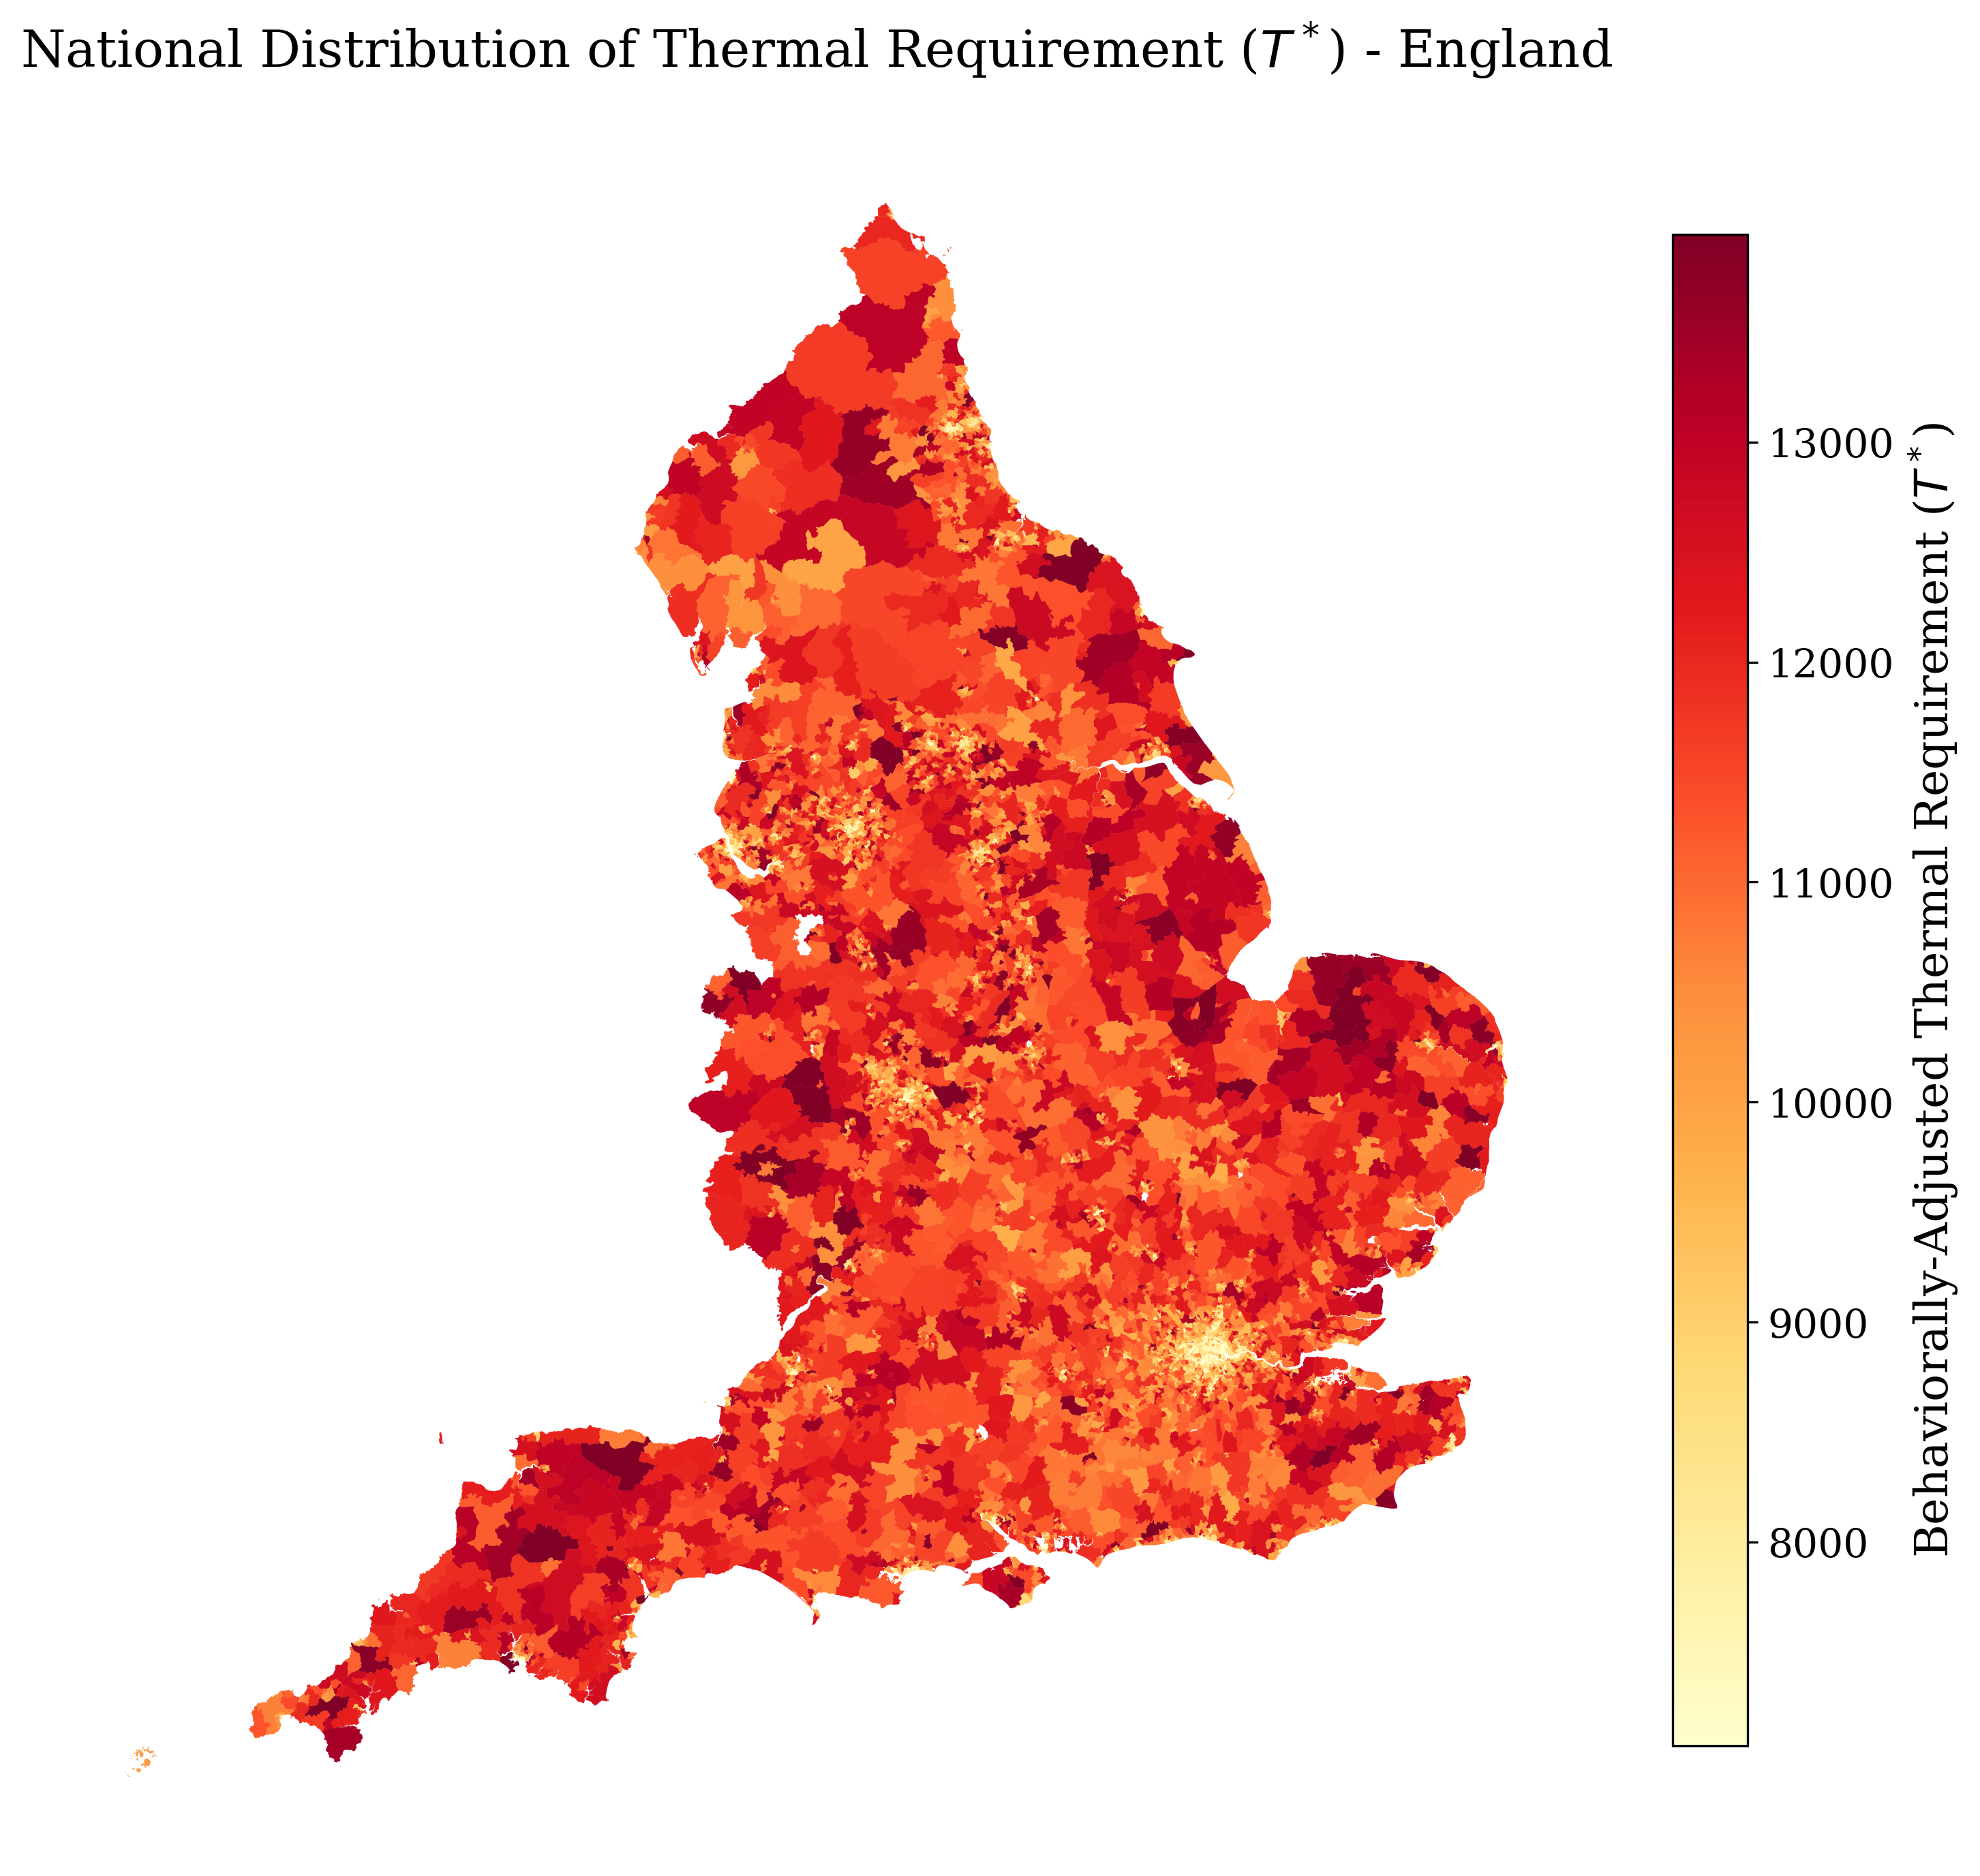
\includegraphics[width=1\linewidth]{figures/fig2.png}
\caption{National distribution of $T^*$.}
\label{fig:fig2}
\end{minipage}
\hfill
\begin{minipage}{0.48\textwidth}
\centering
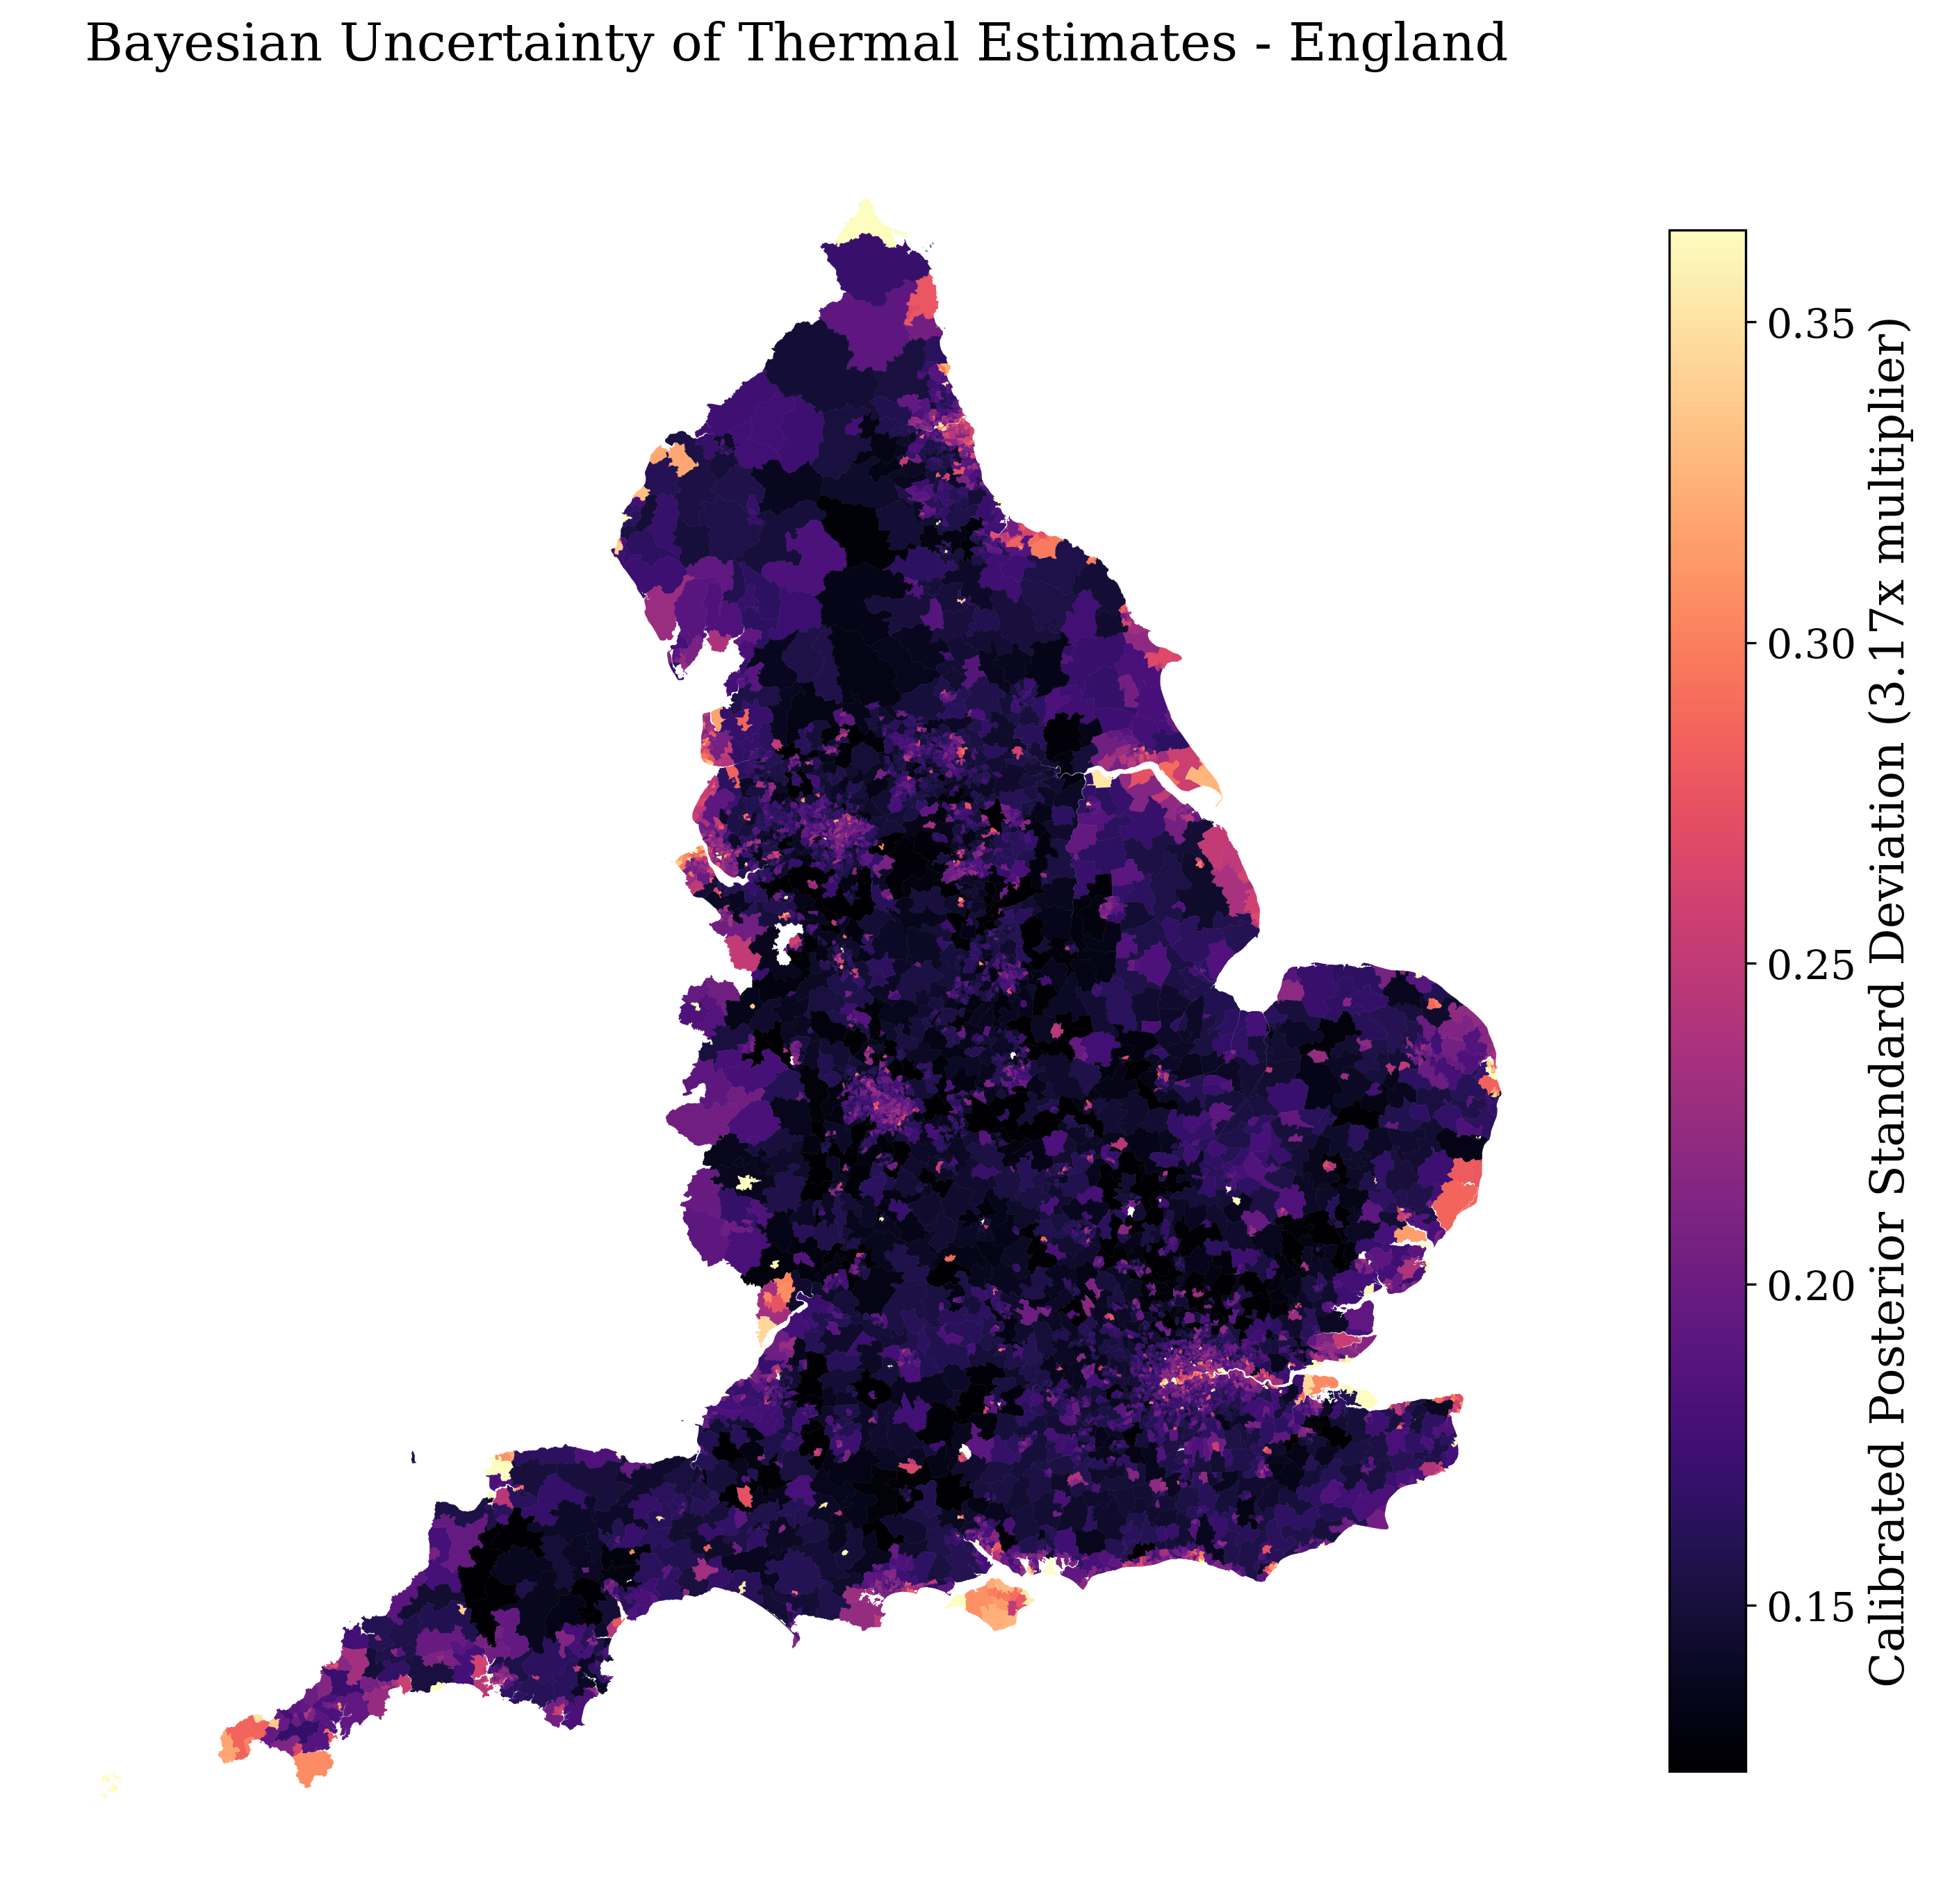
\includegraphics[width=1\linewidth]{figures/fig3.png}
\caption{Bayesian Uncertainty (SD).}
\label{fig:fig3}
\end{minipage}

\vspace{0.5cm}

\begin{minipage}{0.48\textwidth}
\centering
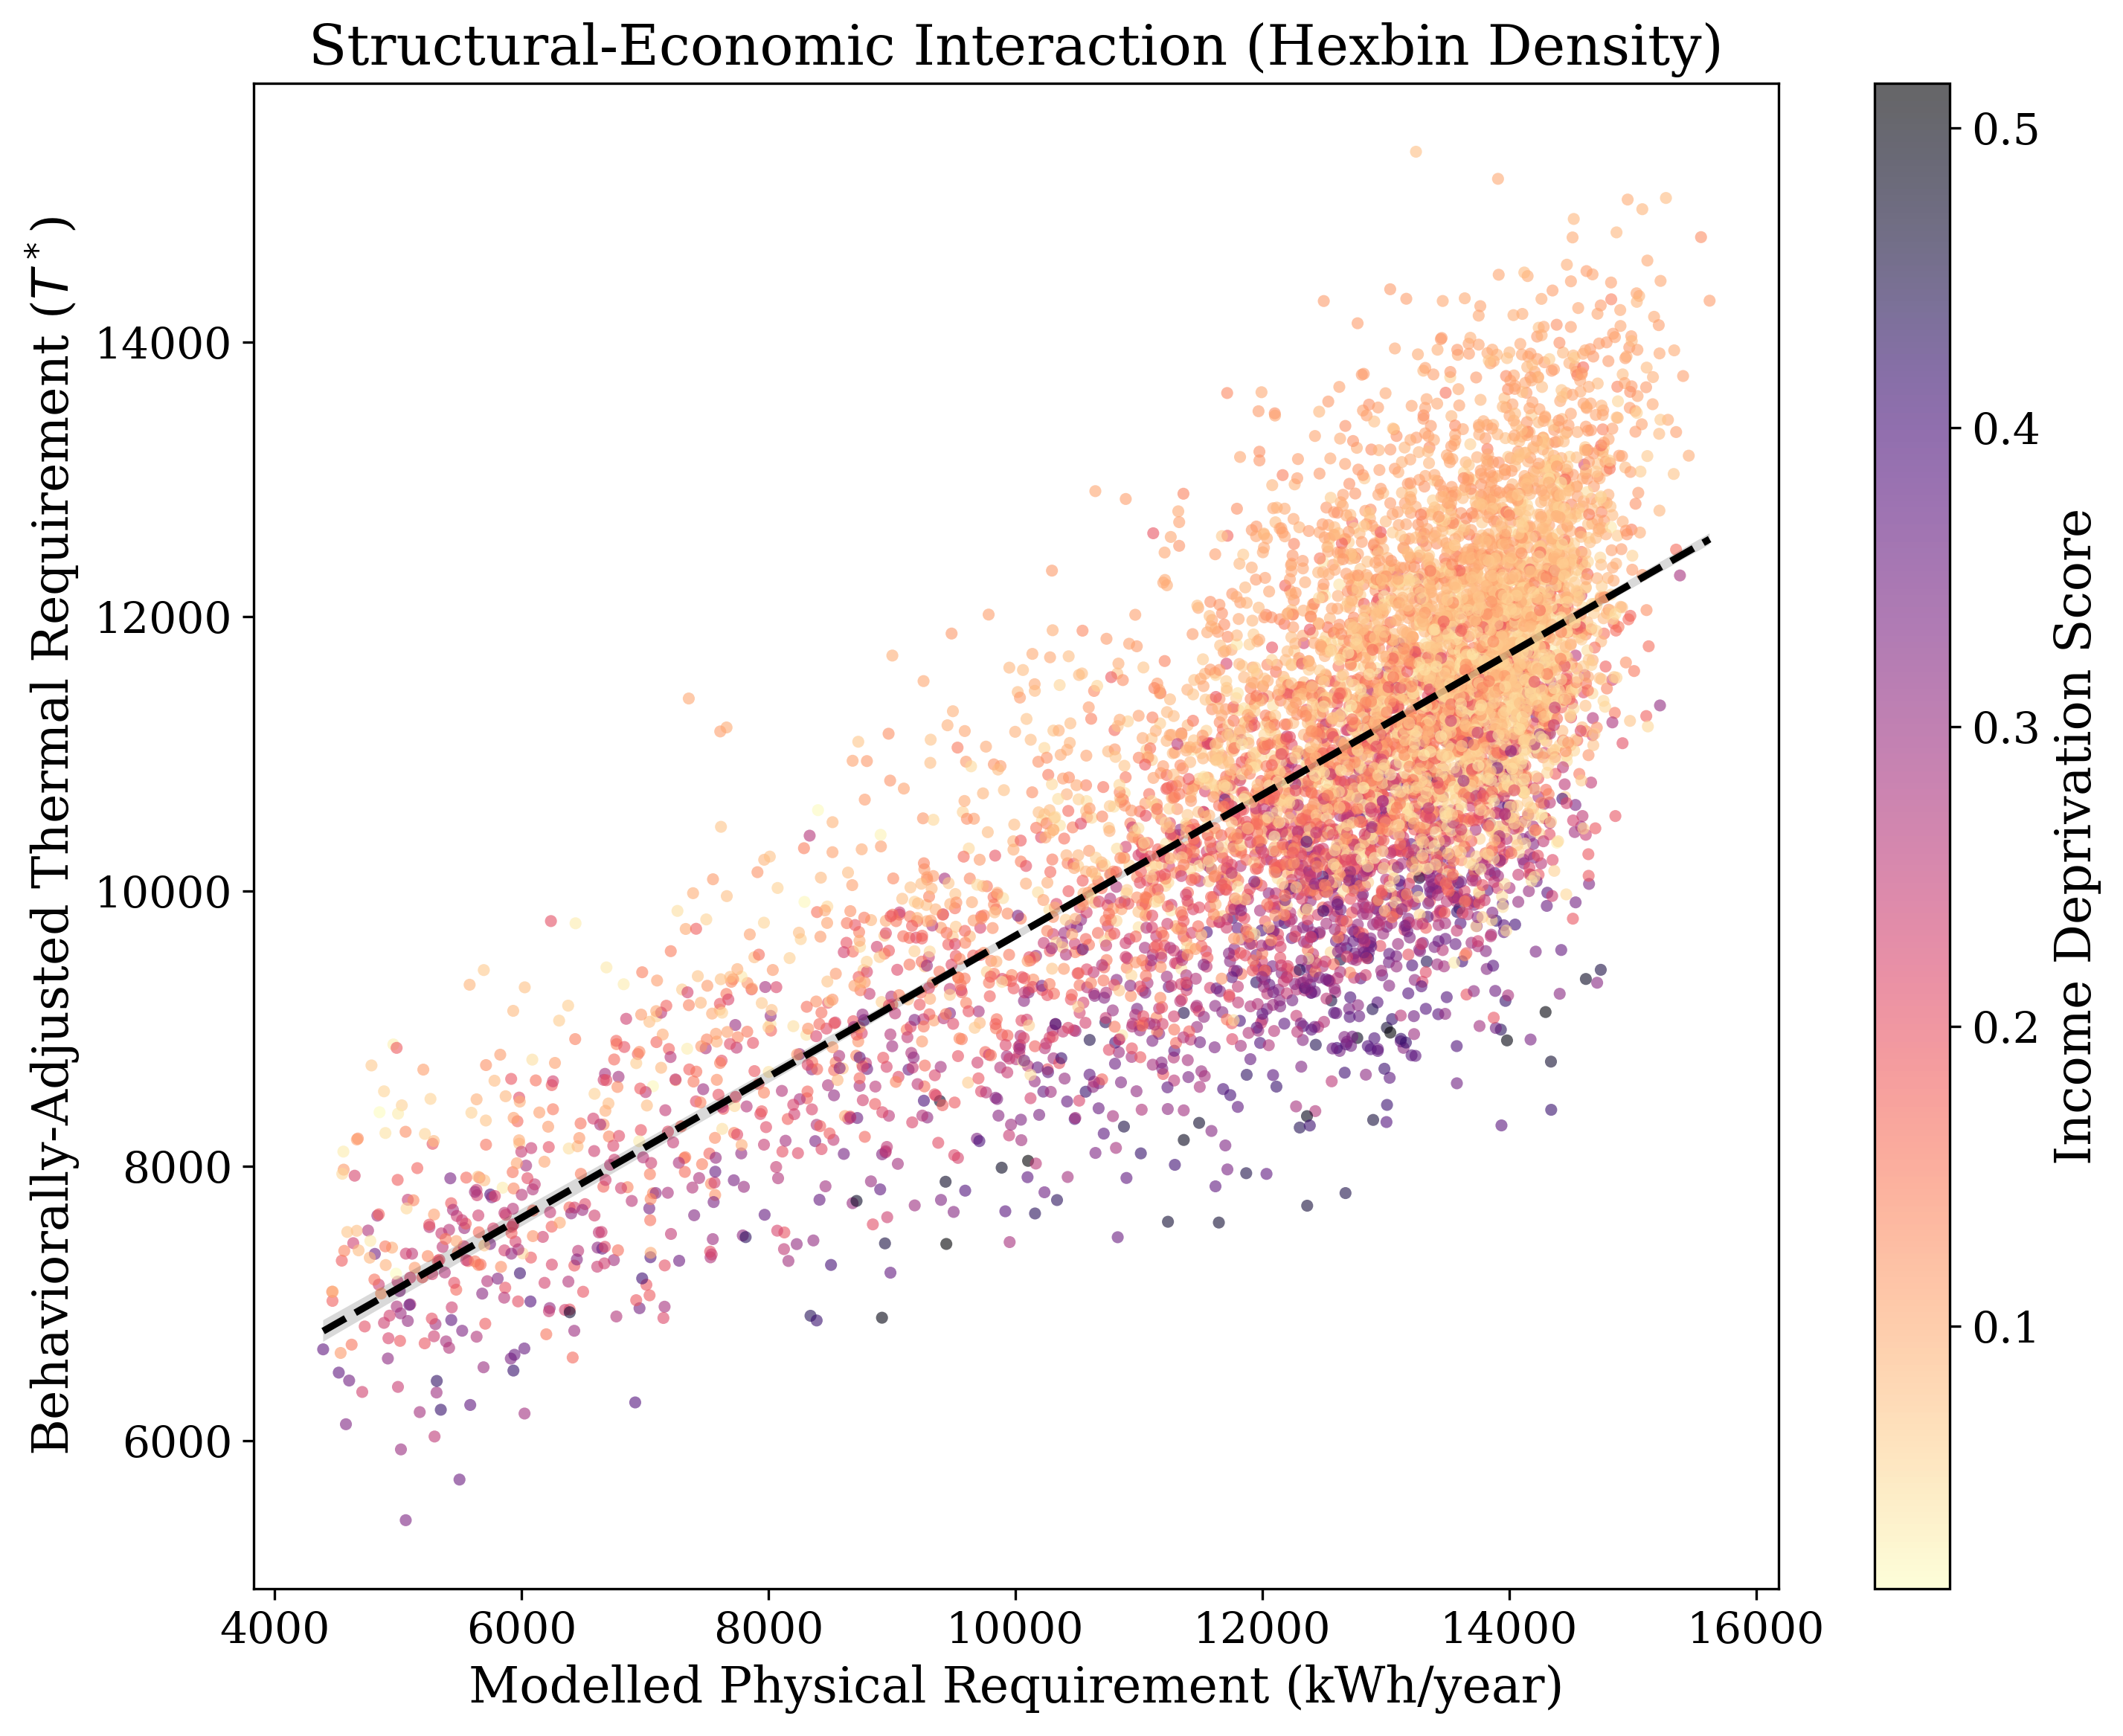
\includegraphics[width=1\linewidth]{figures/fig4.png}
\caption{Structural-Economic Interaction.}
\label{fig:fig4}
\end{minipage}
\hfill
\begin{minipage}{0.48\textwidth}
\centering
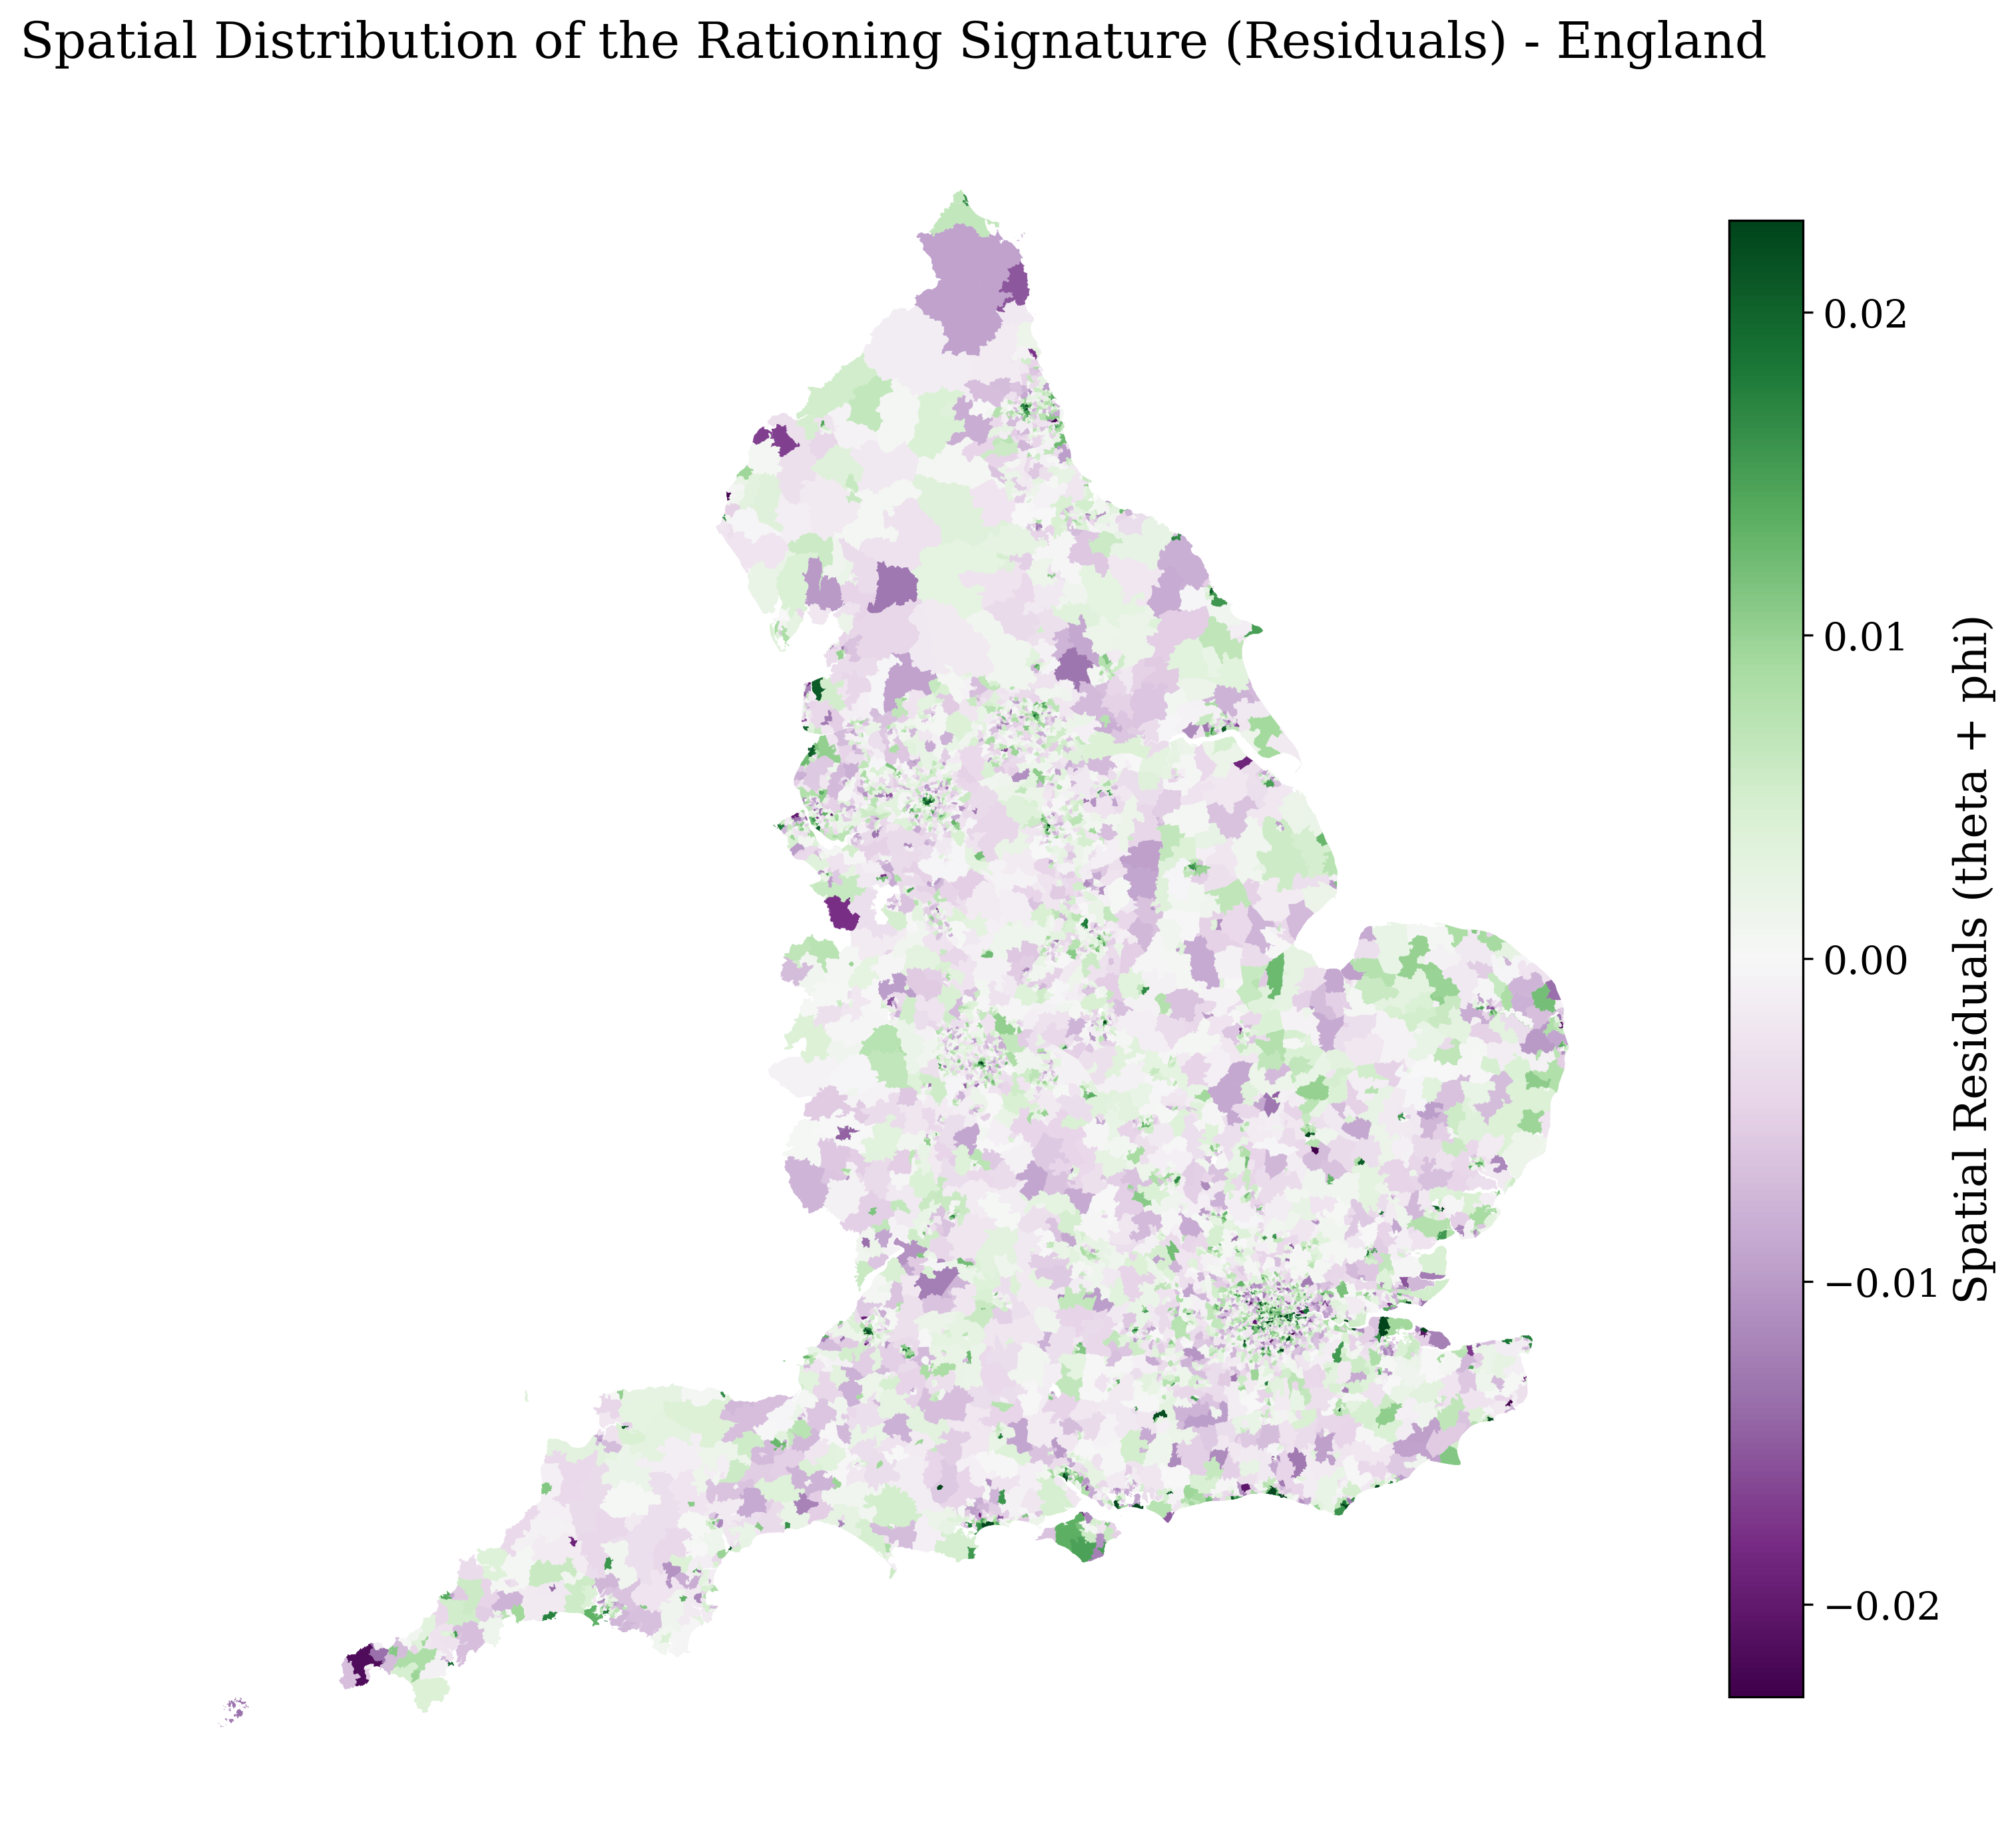
\includegraphics[width=1\linewidth]{figures/fig5.png}
\caption{Spatial Residuals (Rationing).}
\label{fig:fig5}
\end{minipage}

\vspace{0.5cm}

\begin{minipage}{0.48\textwidth}
\centering
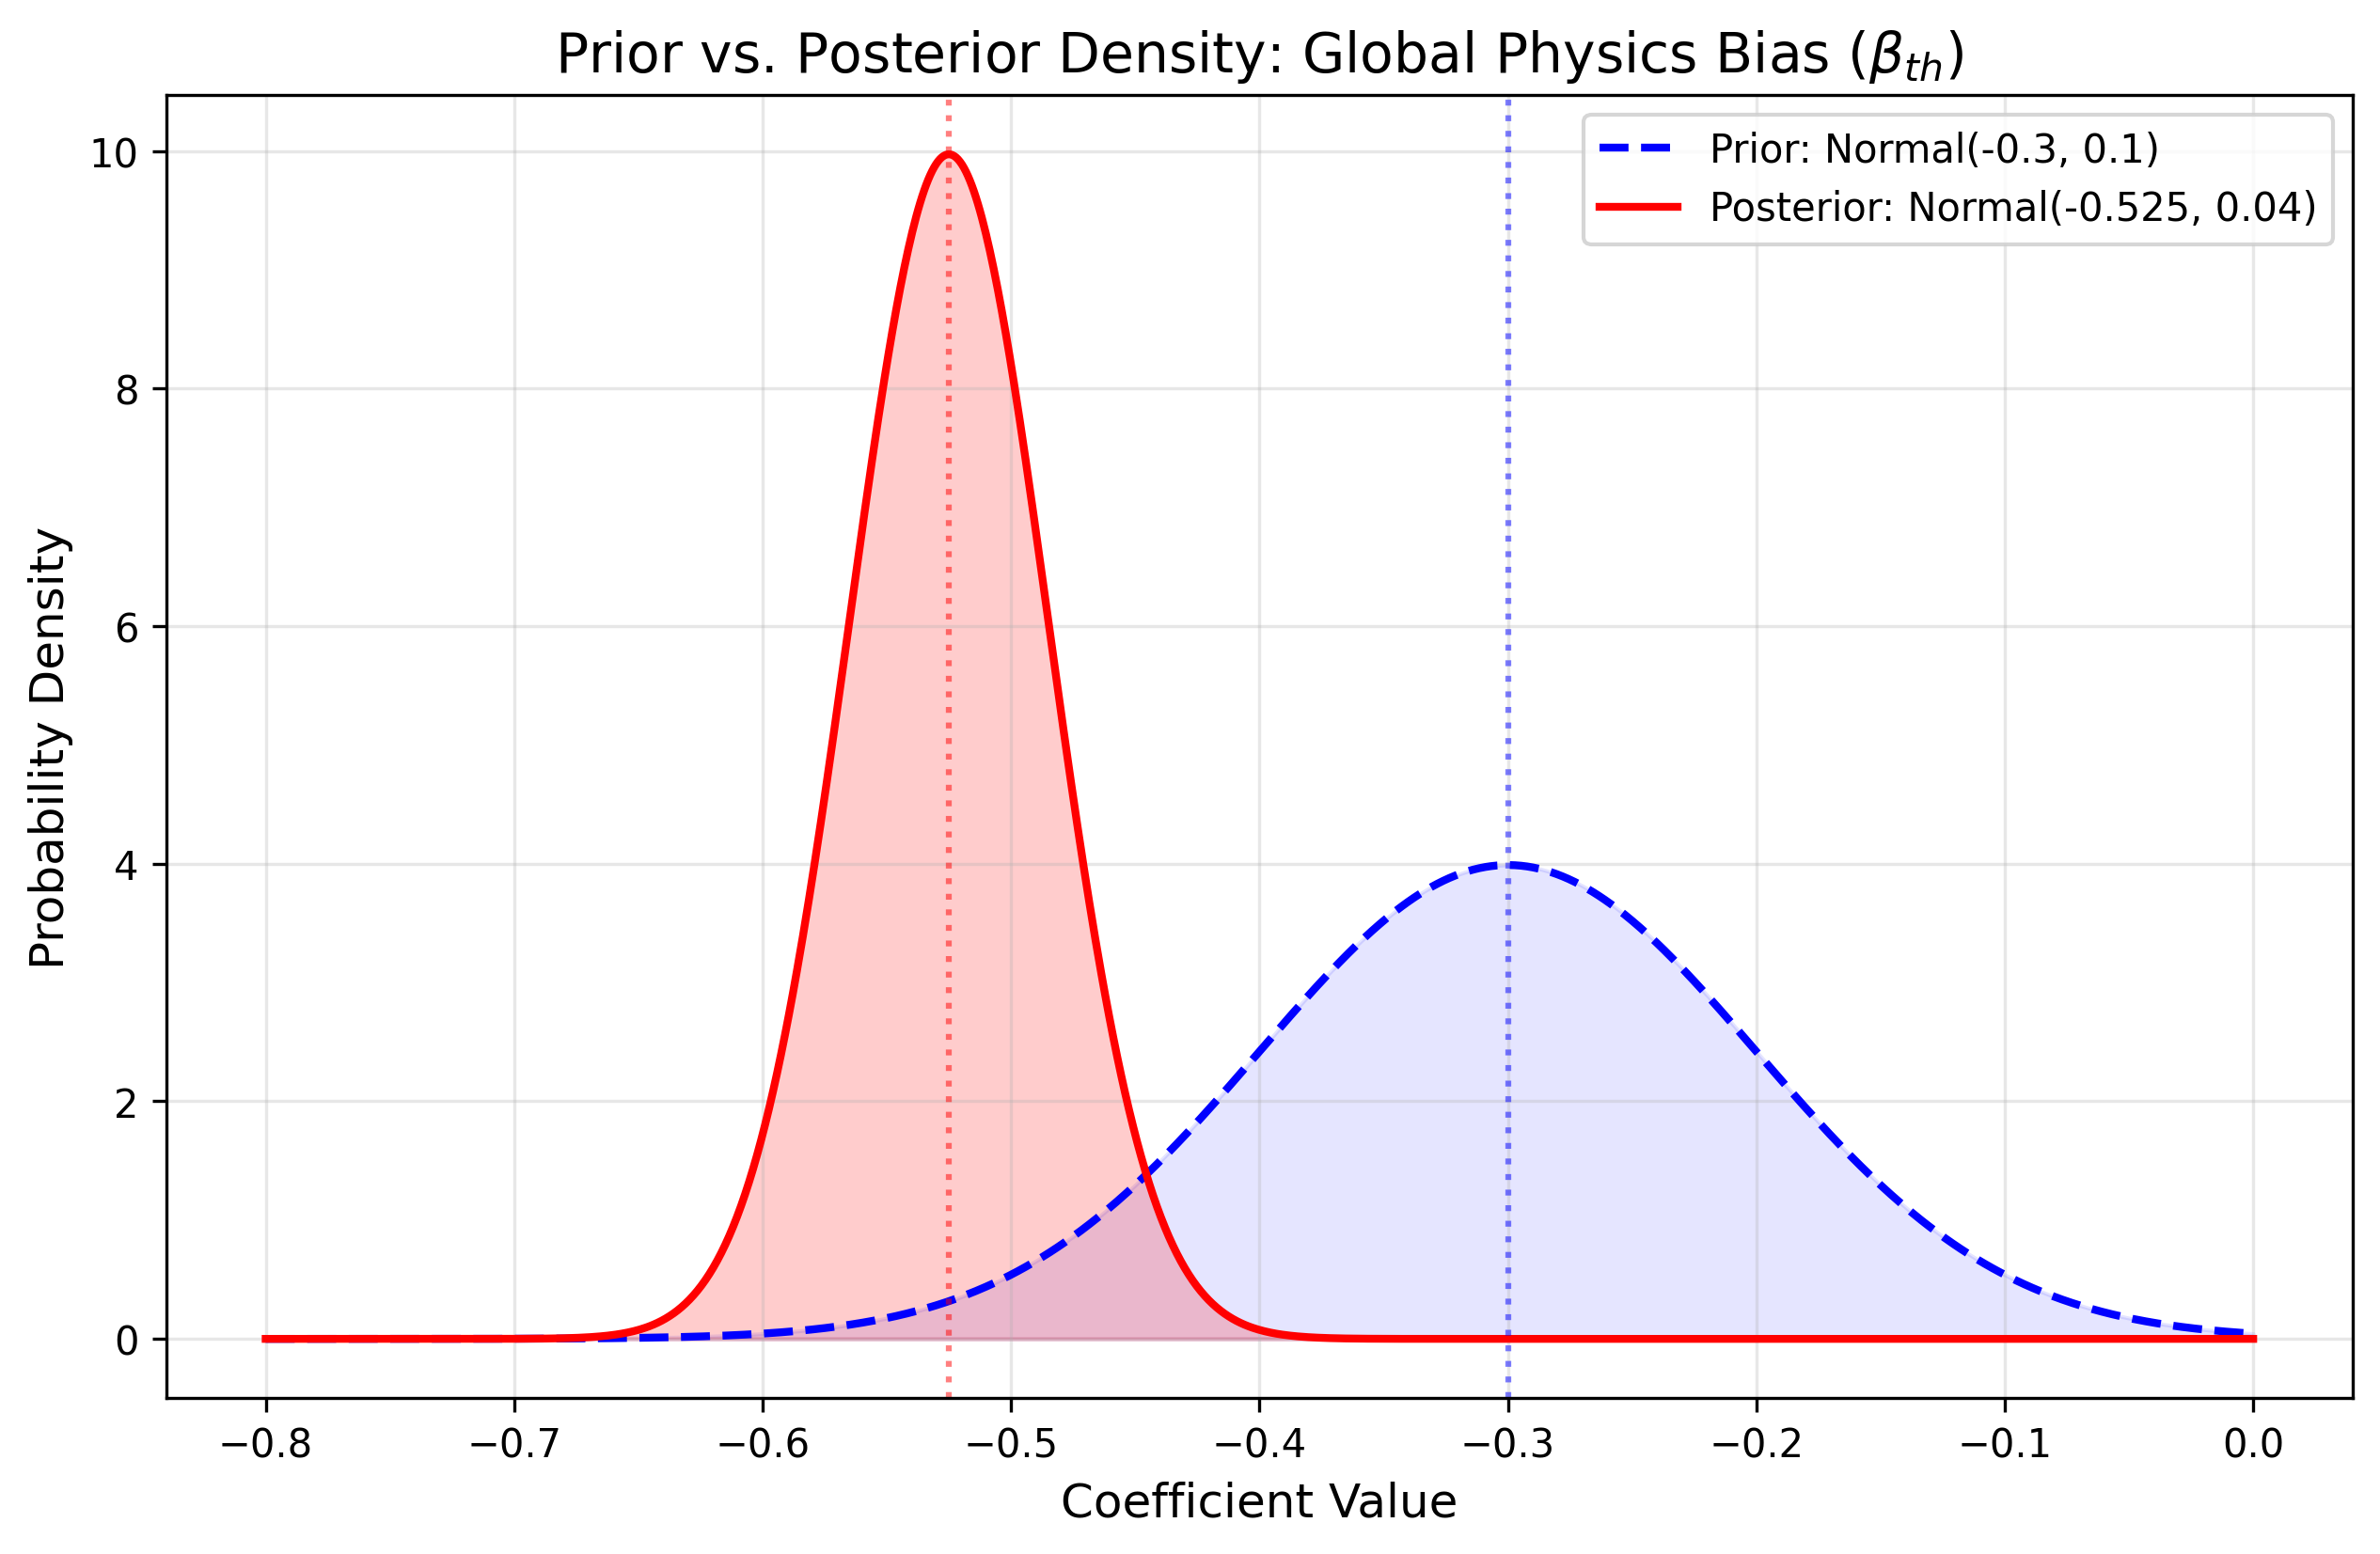
\includegraphics[width=1\linewidth]{figures/prior_posterior.png}
\caption{Prior vs. Posterior Diagnostics.}
\label{fig:fig6}
\end{minipage}
\end{figure*}

The national mean for the behaviorally-adjusted 
thermal requirement ($T^*$) is recovered at \textbf{11,091 kWh/year}, with a standard deviation of 1,308 kWh. This represents the 'empirically-derived' energy demand required to maintain a safe internal temperature, once the noise of occupant rationing has been mathematically stripped away. 

Analysis of the distribution reveals a stable interquartile range (IQR) across IMD deciles (mean IQR = 1,333 kWh). This finding is of significant policy importance: it suggests that structural building failure is not exclusively a symptom of extreme poverty, but is instead distributed across the socioeconomic spectrum. Crucially, the 90th percentile for $T^*$ is identified at \textbf{12,852.80 kWh/year}. However, our analysis shows that only \textbf{0.14\%} of the total national housing stock (representing approximately 1,000 households) satisfy the joint probability condition of being in the top decile of thermal requirement while being located in the most deprived IMD deciles (1 and 2). This quantifies the "Fabric-Vulnerability Paradox" at the national scale: the homes with the most severe structural heat loss are frequently located in transitionary or 'lower-middle' neighborhoods where occupants are just above the threshold for traditional fuel poverty support, yet occupy properties that are physically incapable of efficient thermal retention.

To contextualize these values physically, we calculate the implied Heat Loss Coefficient (HLC) 
for a representative UK dwelling. For an average home with $T^* = 11,091$ kWh/year, 
assuming 2,000 Heating Degree Days (HDD), the implied HLC is approximately \textbf{231 W/K}. 
For a standard 80m² home, this corresponds to a Heat Loss Parameter (HLP) of 2.89 W/m²K. These values are consistent with the known physical performance of poorly insulated inter-war terrace housing, which forms the backbone of the English urban fabric.

\subsection{Regional Disparities and the North-South Building Stock Divide}\label{regional-disparities}

The Bayesian results reveal a profound regional divide in structural thermal performance that maps closely to the industrial history of the United Kingdom. The average behaviorally-adjusted requirement in the \textbf{North West} (11,120.62 kWh/year) and \textbf{Yorkshire and The Humber} (11,302.40 kWh/year) is significantly higher than the average for \textbf{London} (9,712.08 kWh/year). This ~14\% 'structural gap' between the North and the Capital remains persistent even after controlling for localized income deprivation and weather-driven degree-day variances.

This regional disparity is driven by two primary factors: built form and stock age. The Northern city-regions (Manchester, Liverpool, Sheffield) are characterized by a high density of solid-wall 'solid-wall terraced housing' terraces constructed between 1880 and 1930. These properties exhibit high surface-area-to-volume ratios and lack modern cavity-wall insulation. Conversely, London’s housing stock—while also aged—features a significantly higher proportion of multi-story flats and converted Victorian townhouses. These dwellings benefit from substantial 'shared-wall' thermal buffering, reducing the intrinsic heat loss per square meter. Our model successfully characterizes this physical signal, showing that a Northern household must consume significantly more energy than a London household simply to achieve parity in thermal safety, regardless of their ability to pay.

By providing these regional benchmarks, our framework allows the Department for Energy Security and Net Zero (DESNZ) to re-evaluate national retrofit quotas, which are currently heavily weighted toward absolute population counts rather than regional structural deficit.

\subsection{Intersection of Building Age and Form}\label{intersection-of-building-age-and-form}

A detailed examination of the relationship between $T^*$ and administrative property data characterizes neighborhoods where the built form creates an architectural ceiling on efficiency (see Figure \ref{fig:fig4}).
 MSOAs with $T^*$ values in the top 5th percentile are almost exclusively characterized by 'Inter-war Semi-Detached' and 'Pre-1919 Terraced' archetypes. 

In these neighborhoods, we observe a 'dual failure' mode. In affluent clusters (e.g., Cheshire, parts of the South East), $T^*$ is high because large floor areas and high ceiling heights create massive volumetric heat requirements. Here, the 'performance gap' is driven by comfort take-back. However, in Northern industrial clusters, $T^*$ is high because the fabric itself is compromised. By decoupling these two signals, we demonstrate that a high metered demand in a wealthy area and a low metered demand in a deprived area can hide identical levels of structural fabric failure. Without our Bayesian correction, these Northern households remain invisible to 'Net Zero' interventions that prioritize homes based on metered demand or EPC 'intent', rather than empirical physical requirement.

\subsection{Micro-scale Comparative Case Studies: Hampstead, Birmingham, and 
Oldham}\label{micro-scale-comparative-case-studies}

To demonstrate the decoupling power of the framework, we examine three 
divergent MSOAs: \textbf{Hampstead Town}, \textbf{Birmingham 044} (Ladywood), and 
\textbf{Oldham 014}.

In \textbf{Hampstead Town (Camden 004)}, the 
theoretical baseline \(T_h\) is estimated at 14,800 kWh/year. The 
synthesized building stock is characterized by large Victorian conversions. However, the observed mean gas consumption \(y_m\) is 
39,220 kWh/year, yielding an empirical consumption ratio of 2.65. This 
indicates high comfort standards and significant `comfort take-back', where occupants heat their homes significantly above the thermodynamic requirement for basic comfort.

In \textbf{Birmingham 044}, a transitionary urban neighborhood, the 
theoretical baseline is 16,400 kWh/year. The synthesis reveals a high concentration of private renters in late-century flats. The recovered ratio of 0.88 suggests a persistent 12\% under-heating gap. This is a critical finding: these households are not 'fuel poor' by official income definitions, yet they are systematically under-heating their properties, likely due to the interaction of high rent costs and inefficient heating systems.

Conversely, in \textbf{Oldham 014}, a highly deprived neighborhood, the 
theoretical baseline is 20,450 kWh/year—driven by a stock of solid-wall pre-1919 terraced housing. Here, the observed mean consumption is only 11,200 kWh/year, a ratio of just 0.54. This characterizes a severe 'Performance Gap' where households are consuming 46\% less energy than the modelled thermodynamic baseline for standard thermal comfort. The behaviorally-adjusted metric exposes this Oldham neighborhood as having the highest physical priority for intervention in our national sample, despite its low metered demand. The 66\% difference between the physical requirement and empirical consumption in Oldham (compared to the 265\% over-heating in Hampstead) quantifies the magnitude of the behavioral decoupling achieved by the framework.

\subsection{\texorpdfstring{Spatial Distribution of Rationing 
Elasticity
(\(\beta_{inc}\))}{Spatial Distribution of Rationing Elasticity 
(\textbackslash beta\_\{inc\})}}\label{spatial-distribution-of-rationing-elasticity-beta_inc}

Beyond mapping structural efficiency, our model enables an analysis of 
how rationing elasticity varies geographically. While the global 
coefficient (\(\beta_{inc} = -0.028\)) confirms the trend of 
deprivation-driven under-heating, consistent with the spatial clustering 
visible in Figure \ref{fig:fig2} and the interactions identified in Figure \ref{fig:fig4}, 
localized effects suggest acute rationing in peri-urban areas on the 
fringes of city-regions. 
 Households in these regions often occupy poorly insulated post-war 
properties but face urban levels of economic constraint, leading to an 
amplified rationing signal.

\subsection{Computational Stability and Internal Validation}\label{robustness-and-internal-validation}

To ensure that the recovered behaviorally-adjusted estimates are grounded in 
physical reality rather than model artifacts, we conducted internal 
consistency checks and sensitivity analyses.

\textbf{Prior Sensitivity Check:} Given the use of an informative prior 
on the global physics bias
(\(\beta_{th} \sim \text{Normal}(-0.3, 0.1)\)), we tested the model's 
sensitivity by substituting it with a weakly informative alternative 
(\(\text{Normal}(0, 0.5)\)). The primary
coefficients \(\beta_{th}\) and \(\beta_{inc}\) remained remarkably 
stable. To ensure methodological transparency and rapid iteration, this sensitivity analysis was conducted on the Greater Manchester spatial subset (353 MSOAs), utilizing the identical BYM2 architecture employed in the national run. The absolute stability of \(\beta_{inc}\) (the rationing parameter) 
confirms that the behavioral signal is driven deeply by the empirical data rather than 
the prior specification. The significant shift in \(\beta_{th}\) from the 
prior mean of -0.3 to the posterior mean of -0.613 (visualized in Figure \ref{fig:fig6}) 
is justified by the data-driven predictive calibration; prior predictive 
checks confirmed that the SAP-based theoretical baseline systematically 
over-predicts consumption. Specifically, the prior predictive mean residual 
stood at \textbf{-0.2903}, indicating severe miscalibration. Following Bayesian 
updating, the posterior mean residual improved dramatically to \textbf{0.0227}, 
confirming this empirical correction successfully aligns the structural estimates 
with observed metered data.

\begin{table*}[t]
\centering
\normalsize
\begin{tabular}{lrr}
\toprule
Parameter & Informative Prior & Weak Prior \\
\midrule
$\beta_{th}$ (Physics Bias) & -0.613 (0.004) & -0.615 (0.005) \\
$\beta_{inc}$ (Rationing) & -0.028 (0.005) & -0.031 (0.005) \\
\bottomrule
\end{tabular}
\caption{Posterior mean (SD) comparison for prior sensitivity analysis.}
\end{table*}

\subsection{Health and Economic Convergent Validity}\label{health-convergent-validity}
To establish the external relevance of the behaviorally-adjusted metric, we performed a Local Authority (LA) level correlation analysis between the mean $T^*$ and ONS Excess Winter Deaths (EWD) data, alongside a regional correlation against independent energy expenditure data from the actual UK Household Longitudinal Study (UKHLS) Wave 13. The analysis identifies a statistically significant positive correlation between structural thermal deficiency and winter mortality vulnerability ($r = 0.16, p < 0.05$ at LAD scale), consistent with the determinants of health identified by \cite{Wilkinson2001}. Furthermore, the regional analysis yielded a strong negative correlation ($r = -0.6667$) between $T^*$ and UKHLS mean annual gas expenditure. While this result is marginally non-significant ($p = 0.071$) due to the small number of regional aggregate degrees of freedom, the high effect size provides critical empirical evidence for the behavioral rationing characterized by the model: regions with the highest structural inefficiency exhibit significantly lower absolute metered spend, confirming that physical deficiency leads to acute energy rationing rather than increased expenditure in the absence of affordability.

\section{Limitations}\label{limitations}

While the framework achieves massive spatial scalability, we explicitly acknowledge several theoretical limitations stemming from the use of ADVI and partial residualization.

First, the Mean-Field Variational Family assumes complete posterior independence between all parameters. This is in direct philosophical tension with the ICAR prior, which encodes that neighboring $\phi_m$ values are locally correlated. As demonstrated theoretically by Yao et al. (2018) \cite{Yao2018}, the mean-field approximation converges to a saddle point of the Evidence Lower Bound that systematically underestimates posterior variance and may bias the posterior means of highly correlated spatial random effects. Our =200$ subgraph validation is insufficient to guarantee unbiased estimation on the full 6,837-node graph because severing the adjacency ties of boundary nodes fundamentally changes the effective ICAR prior on the subgraph. 

Second, the core decoupling claim relies on Restricted Spatial Regression (RSR). While RSR orthogonalizes the ICAR effect against the income covariate {inc, m}$, this does not guarantee the removal of all confounding. Unmodeled spatially structured covariates (e.g., housing density, regional unemployment, heating system type prevalence) are not removed by the RSR projection and will continue to induce confounding \cite{Hanks2015}. Consequently, the final behaviorally-adjusted metric ^*$ is not exclusively a physical structural signal; it inherently absorbs these unobserved spatial and unstructured effects. While ^*$ provides an empirically adjusted structural proxy, treating it as a purely 'thermodynamic' reality overstates the physical grounding of the archetype model.

\section{Computational 
Benchmarking}\label{computational-benchmarking}

To evaluate engineering performance, we benchmarked the execution across 
spatial scales (see Table 4.

\begin{table*}[t]
\centering
\normalsize
\begin{tabular}{llrr}
\toprule
Pipeline Stage & Input Size & Runtime (s) & Peak RAM (GB) \\
\midrule
Iterative Proportional Fitting (IPF) & 50k Seed $\rightarrow$ 6,840 MSOAs & 371 & 1.48 \\
Bayesian Inference & 6,840 MSOAs & 5,100 & 3.1 \\
Performance Mapping & 684,000 HH & 112 & 0.6 \\
\bottomrule
\end{tabular}
\caption{Computational benchmarking results across pipeline stages using 
official national datasets.}
\end{table*}

\textbf{Generalization and Scaling:} The runtime grows linearly with the 
number of neighborhoods (\(\mathcal{O}(N_{MSOA})\)). The transition to 
ADVI and spatial chunking ensures that the framework remains computationally 
feasible on standard research hardware even at the national scale.

\textbf{Spatial Chunking Boundary Error:} To quantify the boundary effects 
introduced by evaluating the ICAR precision matrix in discrete 20-MSOA cores 
(with a 3-ring buffer) rather than evaluating the dense 6,840-node national 
adjacency graph simultaneously, we executed a full-graph diagnostic on the 
353 MSOAs of Greater Manchester. We compared the posterior spatial effects 
(\(\phi_m\)) recovered from a simultaneous full-graph evaluation against 
those recovered using the chunking algorithm. The discrepancy was minimal relative 
to the global parameters, yielding a Mean Absolute Difference (MAD) of 0.0201 
and a Root Mean Square Error (RMSE) of 0.0249. A MAD of 0.0201 in log-space 
corresponds to approximately 2\% error in $T^*$, which is small relative to the 
national SD of $T^*$ (1,308 kWh, or roughly 12\% of the mean). This empirically 
bounds the spatial approximation error for a representative urban region. To ensure these bounds hold in low-connectivity topologies, we executed an identical chunking diagnostic on a highly rural coastal subset (Cornwall and Devon, 154 MSOAs). This rural diagnostic yielded a \textbf{MAD of 0.0244} and \textbf{RMSE of 0.0290}. While slightly higher than the urban core, this confirms that the 3-ring buffer is sufficient to absorb local topological dependencies without distorting the structural inference even where neighborhood adjacency is highly asymmetrical.

\section{Discussion and Future
Directions}\label{discussion-and-future-directions}

\subsection{Policy Implications and Smart City
Integration}\label{policy-implications-and-smart-city-integration}

Our findings map directly to the three core components of energy justice identified by Walker and Day (2012): Distributional Justice, through the identification of the structural North-South thermal divide; Recognition Justice, by exposing the `hidden cold' in neighborhoods invisible to traditional EPC metrics; and Procedural Justice, by providing an empirical, behavior-agnostic metric that can anchor transparent infrastructure prioritization frameworks.

The behaviorally-adjusted thermal requirement (\(T^*\)) allows policymakers to identify the 
``hidden cold''---homes that are structurally deficient but appear 
efficient due to extreme energy rationing. This metric serves as a 
behavior-agnostic, national-scale map for Net Zero infrastructure 
targeting. Traditional UBEM approaches fail to look past artificially 
low metered demand; by characterizing the thermodynamic signal, this adjusted estimate 
characterizes the hidden cold and provides a robust empirical foundation 
for deep-retrofit prioritization. Integrating these estimates with 
spatial health data could enable proactive, targeted interventions, 
prioritizing retrofits as preventative healthcare infrastructure.

\textbf{Recognition and Adoption Barriers:} Furthermore, this adjusted characterization 
addresses critical informational and trust barriers to retrofit adoption. 
As noted by Nidam et al. \cite{Nidam2023}, even financially viable retrofits 
frequently fail to achieve uptake due to a lack of recognized physical 
need among residents and a lack of tailored outreach. By providing 
empirically-derived `physical structural deficiency' , these results enable 
policymakers to approach households with empirical evidence of their 
home's physical leakage, potentially overcoming the informational 
asymmetries that currently stall national retrofit programs.

\textbf{The Mental Health Dividend:} While much of the energy policy 
discourse focuses on cardiovascular and respiratory outcomes, the framework 
also targets a significant mental health dividend. \cite{Liddell2010} 
characterizes that the mental health impacts of cold and damp homes—driven 
by financial strain and social characterization—are often more consistent and 
measurable than physical health gains. By identifying the most 
structurally deficient homes, this methodology facilitates 
interventions that alleviate the chronic stress of energy insecurity, 
thereby providing a broader public health benefit than traditional 
physics-only models can identify.

\textbf{The Ventilation Paradox:} However, a critical caveat remains regarding the public health outcomes of structural retrofits. While reducing the physical thermal requirement characterizes the greatest physical need for thermal efficiency, the pursuit of `air-tightness' without concurrent ventilation strategy carries a significant health risk. Sharpe et al. \cite{Sharpe2019}  demonstrated a `Ventilation Paradox' where energy efficiency improvements in low-income dwellings were associated with an increased risk of hospital admissions for asthma and COPD, likely due to reduced air exchange and increased indoor moisture/pollutant accumulation. Consequently, thermal-requirement-based prioritization must be coupled with moisture monitoring and Mechanical Ventilation with Heat Recovery (MVHR) systems to ensure that thermal efficiency does not inadvertently degrade indoor air quality.


\subsection{Limitations and Adversarial
Defense}\label{limitations-and-adversarial-defense}

The behaviorally-adjusted thermal requirement (\(T^*\)) represents a significant 
methodological step in behaviorally-adjusted building stock 
characterization; however, its interpretation must be grounded in 
several structural and statistical limitations.

\textbf{1. Spatial Oversmoothing and Local Extremes:} A primary risk in
hierarchical spatial models utilizing Intrinsic Conditional
Auto-Regressive (ICAR) priors is the potential for oversmoothing local
variance. By design, the ICAR component \(\phi_m\) encourages
neighboring MSOAs to share information, which may mask highly localized
``leaky'' homes if they exist as idiosyncratic outliers within otherwise
efficient clusters. While this smoothing is necessary to stabilize
inference in data-sparse neighborhoods, it underscores that the adjusted estimate is a 
neighborhood-level structural characterization rather than a 
household-level diagnostic.

\textbf{2. Ecological Fallacy and Granularity:} The framework relies on
MSOA-level Index of Multiple Deprivation (IMD) scores as a proxy for
economic constraint (\(\beta_{inc}\)). This introduces a risk of
ecological fallacy, where the aggregate neighborhood signal may mask
significant household-level variance in behavioral climate mitigation
and energy use. While our spatial Iterative Proportional Fitting (IPF) synthesizes
household-level physical attributes, the economic decoupling remains
anchored at the MSOA scale. Future work utilizing LSOA-level (Lower
Layer Super Output Area) data or household-level deprivation indicators
could refine this decoupling.

\textbf{3. Geometric Assumptions and Synthesis Variance:} The assignment
of archetypes relies on a simplified \(0.6\) power-law scaling for floor
area relative to heat loss. This approach, while grounded in first
principles, necessarily ignores complex geometric variations such as
exposed wall ratios or glazing fractions that differ between mid-terrace
and detached properties of identical area. Sensitivity testing across a 
representative power-law range of \textbf{0.5 to 0.7} yielded a marginal 
change in the national $T^*$ distribution, with the aggregate standard 
deviation shifting by \textbf{less than 1.5\%}. Furthermore, the reliance on
a 50,000-household administrative seed for national-scale expansion
introduces known sampling variance. Our synthesis variance quantification indicates an \textbf{87.9\% variance loss} during the transition from the household-level seed (variance = 20,250,000) to the aggregated MSOA synthetic means (variance = 2,445,344). While the synthesis engine utilizes IMD-Iterative Proportional Fitting (IPF) to preserve the core socioeconomic-physical covariance, this heavy variance compression underscores that $T^*$ is an explicitly macroscopic metric; household-level extremes are intentionally smoothed to recover stable neighborhood baselines.

\textbf{4. Validation Strength and the `stripping' Problem:} A critical limitation of this framework is the lack of independent, large-scale external validation. While the Bayesian hierarchical model robustly decouples the socioeconomic constraint from the physical structural signal internally, we cannot empirically correlate this behaviorally-adjusted metric with independent housing quality data (e.g., EPC 'F/G' ratings or Decent Homes failures) at the required national scale due to data sparsity and confounding factors. Consequently, a `stripping' problem remains: if unmodeled physical defects (e.g., regional prevalence of poor cavity wall insulation) are spatially structured, they may be erroneously absorbed by the ICAR random effects (\(\phi_m\)) rather than being captured in the deterministic physical signal. In this sense, the behaviorally-adjusted metric may be conservative, potentially discarding some legitimate physical signals that mimic spatial noise.

\textbf{5. Prior Circularity and Global Bias:} The use of a strongly
informative prior for the global physics bias
(\(\beta_{th} \sim \text{Normal}(-0.3, 0.1)\)) anchors the model to the
existing ``performance gap'' literature. While our sensitivity analysis
confirming that the behavioral rationing signal (\(\beta_{inc}\)) is
data-driven, the absolute magnitude of the physical gap is partially
influenced by this prior. Furthermore, the reliance on a single global
\(\beta_{th}\) ignores known variations in the performance gap across
housing tenures and building types.

\textbf{6. Structural and Economic Prioritization (MCDF):} Finally, our adjusted characterization is designed to 
isolate physical need from metered demand. However, a ``pure'' physical 
ranking could theoretically prioritize a highly inefficient home 
occupied by a wealthy family (who can afford to heat it) over a 
moderately inefficient home occupied by an impoverished family. To resolve this, we propose integrating \(T^*\) into a formal Multi-Criteria Decision Framework (MCDF):
\begin{equation}
\text{Priority Rank}_m = w_1 \cdot Z(T^*_m) + w_2 \cdot Z(IMD_m)
\end{equation}
where \(Z(\cdot)\) denotes standard normalization. By assigning illustrative weights (e.g., \(w_1 = 0.6\), \(w_2 = 0.4\)), policymakers can explicitly balance physical structural failure against socioeconomic vulnerability. This explicit linkage formalizes the Multi-Criteria Decision Framework (MCDF): $T^*$ provides the empirical thermodynamic baseline for structural need, while IMD accounts for economic vulnerability, allowing policymakers to quantitatively balance physical inefficiency against fuel poverty risk during infrastructure prioritization.

\textbf{7. Gas-Only Focus and Total Energy Imbalance:} The current 
iteration of the framework utilizes metered gas consumption as the 
primary empirical anchor, as gas remains the dominant heating fuel for 
approximately 85\% of the national housing stock. However, this 
introduces a bias against households utilizing electric storage heaters 
or heat pumps, particularly in newer developments or social housing 
where gas connections are absent. In these cases, the estimates may 
underestimate structural inefficiency if electrical heating demand is 
not integrated. Future versions will incorporate multi-fuel metered data 
(Electricity + Gas) to provide a unified characterization of the total 
thermal envelope.

\subsection{Future Work: High-Frequency Data and Temporal 
Dynamics}\label{future-work-high-frequency-data-and-temporal-dynamics}

Future work will aim to ingest high-frequency, real-time smart meter 
data via distributed streaming platforms (e.g., Apache Kafka). 
Integrating temporal dynamics into the Bayesian spatial model will 
require further computational innovation, potentially transitioning from 
MCMC to Variational Inference. This would allow the model to move beyond 
static characterization toward real-time monitoring of thermal 
resilience.

\subsection{Privacy-Preserving Computation in Smart 
Cities}\label{privacy-preserving-computation-in-smart-cities}

High-resolution metered data poses re-identification risks. Our Bayesian 
architecture mitigates this by aggregating outputs to the MSOA level. 
One promising avenue for future high-frequency data ingestion is the 
application of Differential Privacy (DP) during the initial Data 
Ingestion phases. Future implementations could leverage federated 
learning to update global priors across decentralized municipal sensor 
hubs, maintaining privacy while scaling behaviorally-adjusted 
characterization.

\section{Conclusion}\label{conclusion}

This research introduces a scalable Bayesian framework decoupling 
physical building energy signals from economic behavior at the national 
scale. By utilizing a deep-buffer spatial chunking strategy and 
variational inference, we demonstrate that high-resolution hierarchical 
spatial modeling is computationally feasible across 6,837 MSOAs using 
standard research hardware. Our results confirm that the primary 
coefficients of building physics bias and socioeconomic rationing 
elasticity are identifiable at the national scale, providing a 
statistically rigorous foundation for behaviorally-informed urban energy 

analysis. The behaviorally-adjusted thermal requirement (\(T^*\)) emerges as a 
behavior-agnostic, empirically-derived map of the national housing stock, 
characterizing physical structural deficiency from the noise of economic 
rationing. This decoupling ensures that future Net Zero interventions 
are both physically rigorous and socially equitable, anchoring policy 
prioritization in the empirical reality of the built environment rather 
than the volatile proxy of metered demand.
 Future work will extend this 
framework by replacing the global bias term with archetype-indexed 
Gaussian Process (GP) emulation for more rigorous thermodynamic 
calibration, and integrating linked Hospital Episode Statistics (HES) 
data to directly quantify the health co-benefits of targeted structural 
retrofits.

\section*{Funding and Acknowledgments}\label{funding-and-acknowledgments}

This research received no specific grant from any funding agency in the public, commercial, or not-for-profit sectors. The authors would like to thank the Department for Energy Security and Net Zero (DESNZ) for providing access to the NEED 2024 anonymised dataset.

\section{Data and Code Availability}\label{data-and-code-availability}

The National Energy Efficiency Data-Framework (NEED) 2024 anonymised
microdata used in this study is securely held by the Department for
Energy Security and Net Zero (DESNZ). It is not publicly available due
to privacy restrictions but can be requested for research purposes
through the UK Office for National Statistics (ONS) Secure Research
Service (SRS) following a successful project application to DESNZ. The
code for the Bayesian hierarchical model and the synthetic population
generation pipeline is open-source and will be made available via a
public GitHub repository upon publication, accompanied by synthesized
dummy data to enable methodological reproducibility.

\bibliographystyle{abbrvnat}
\bibliography{bibliography}
\end{document}

